\documentclass[14pt,oneside,titlepage,reqno,a4paper]{book}%{book}%%{these_gi}%twosidedraft,
\usepackage{xkeyval}
\usepackage{titlesec}
\usepackage{times} 
\usepackage{amsmath} 
% Định nghĩa thuật toán
%Tạo Index
\usepackage{algorithm}
\usepackage{algorithmic}
\usepackage{multirow}
\usepackage{makeidx}
%Thụt vào đầu dòng mỗi đoạn
\usepackage{indentfirst}
\setlength{\parindent}{1cm} 
%\input setbmp
%Để chế độ thụt vào đầu dòng trong chế độ liệt kê số (enumerate)
 \usepackage{enumitem} 
% \usepackage{lipsum} 
 \setlist[enumerate]{itemindent=\dimexpr\labelwidth+\labelsep\relax,leftmargin=1em} 
% \setlist[itemize][label =-]{itemindent=\dimexpr\labelwidth+\labelsep\relax,leftmargin=1em} 
\setlist[itemize,1]{label=-}%thay vì dấu chấm thì là dấu gạch đầu dòng
 %
 %Thụt vào đầu dòng đối với tiêu đề của section


\setcounter{secnumdepth}{5} %Đặt chiều sâu của các section. Với số 5, ta có đến paragraph
\renewcommand\thesection{\bfseries \arabic{section}.}
%\renewcommand\thesection{\Roman{section}.} %Đặt số thứ tự của Section là I, II, III
% Cài đặt độ sâu cho tiêu đề: Ở đây là chương rồi đến mục
\renewcommand\thesubsection{\arabic{section}.\arabic{subsection}.} %Đặt số thứ tự của subseciton là 1., 2., 
\renewcommand\thesubsubsection{\alph{subsubsection})} %Số thứ tự của subsubsection là a), b)
%
%\titleformat{\section}[runin]{\bfseries}{\thesection}{1em}{} %Cho phép chữ đi ngay sau tiêu đề. Cái này không dùng ở đây.
\titleformat{\section}[block]{\normalfont}{\thesection}{.5em}{ \bfseries }
% Đặt cỡ chữ cho tiêu đề : \large: cớ lớn; \bfseries: là đậm
%\titleformat{\section}[block]{\normalfont}{\thesection}{.5em}{\MakeUppercase}% Cài đặt form của section\bfseries. Makeuppercase là để chữ in hoa cho section
\titlespacing{\section}{2em}{.5em}{.5em}%Khoảng cách section đến đầu dòng: thụt vào 2em = 1cm
\titleformat{\subsection}[block]{\bfseries}{\thesubsection}{.5em}{}%Tương tự section\itshape
\titlespacing{\subsection}{2em}{.5em}{.5em}
%==============Hằng thêm vào
\titleformat{\subsubsection}[block]{\bfseries}{\thesubsection}{.5em}{}%Tương tự section\itshape
\titlespacing{\subsubsection}{2em}{.5em}{.5em}
%=====================
%Chú ý: \bfseries là chữ đậm, \itshape là chữ nghiêng.
\titleformat{\subsubsection}[block]{\bfseries\itshape}{\thesubsubsection}{.5em}{}
\titlespacing{\subsection}{2em}{.5em}{.5em}
%

%\usepackage[absolute]{textpos} 
%\usepackage{cases}
\usepackage{hyperref}		%Tạo liên kết từ mục lục tới các phần tương ứng
\usepackage[mathscr]{eucal}%
\usepackage[nottoc]{tocbibind}

%\RequirePackage{refcount}[2006/02/12]
%\usepackage{pstricks}

\usepackage[utf8]{vietnam}
%\documentclass[a4paper, 14pt]{report}
%\usepackage[utf8]{vntex}
%\input{macros}
\usepackage{scalefnt}
\usepackage[left=3.0 cm, right=2 cm, top=2.5 cm, bottom=2.5 cm]{geometry}%tạo lề của trangleft=3.5 cm, right=2.5 cm, top=2.5 cm, bottom=2.5 cm]
\usepackage{graphicx}
\usepackage{wrapfig}
\usepackage{amsmath,amsthm,array}%
\usepackage{slashbox}
%==================
% Fancy style
%======================
\usepackage{fancyhdr}
\pagestyle{fancy}

%\renewcommand{\chaptermark}[1]{\markboth{#1}{}}
\renewcommand{\sectionmark}[1]{}%\markright{\Roman{section}.\ #1}}

\renewcommand{\headrulewidth}{0.4pt}%Tạo bề dày của các đường thẳng chia header, footer
%\renewcommand{\footrulewidth}{0pt}
\fancyhead{}
\fancyfoot{}
\fancyhead[RO,LE]{\normalsize\itshape{{\nouppercase{\rightmark}}}}
\fancyhead[LO,RE]{\normalsize\itshape{{\nouppercase{\leftmark}}}}
\fancyfoot[C]{{\normalsize{\thepage}}}
%\fancyfoot[LO,LE]{\textbf{{\normalsize{Lý thuyết thông tin - Phạm Văn Cảnh, Phạm Thị Hằng, Lê Huy Dũng}}}}
%=======Các Định lý, Định nghĩa, Bổ đề, Hệ quả =======

 
%\newtheorem{vd}{Ví dụ}[section]
\newtheorem{theo}{Định lý}[chapter]
\newtheorem{lem}{Bổ đề}[chapter]%[section]
\newtheorem{coro}{Hệ quả}[chapter]%[section]
\theoremstyle{definition}
\newtheorem{dn}{Định nghĩa}[chapter]%[section]
\newtheorem{define}{Định nghĩa}[chapter]
\floatstyle{ruled}
\newfloat{algorithm}{htbp}{loa}
\floatname{algorithm}{Thuật toán}

\renewcommand{\thedn}{\arabic{chapter}.\arabic{dn}}%
%\newenvironment{proof}[1][Chứng minh.]{\begin{trivlist}
%\item[\hskip \labelsep {\bfseries#1}]}{\end{trivlist}}
\newenvironment{vd}[1][Ví dụ.]{\begin{trivlist}
\item[\hskip \labelsep {\bfseries#1}]}{\end{trivlist}}

\newtheorem{example}{Ví dụ}[chapter]
\newenvironment{remark}[1][Chú ý.]{\begin{trivlist}
		\item[\hskip \labelsep {\bfseries#1}]}{\end{trivlist}}

%Khoảng cách giữa các đoạn, cách dòng, giãn dòng
\setlength{\baselineskip}{5truept} 
%\renewcommand{\baselinestretch}{1.3}%Cách dòng 1.2
\linespread{1.3}
%\abovedisplayskip =6pt plus 6pt minus 9pt
%\abovedisplayshortskip =0pt plus 6pt minus 9pt
\belowdisplayskip =\abovedisplayskip
\belowdisplayshortskip =\abovedisplayshortskip


%\scalefont{1.4}
%\fontsize{13pt}{20pt}\selectfont
%\fontsize{13pt}{22pt}{\selectfont}
%\parindent=0pt
%=================Đánh số cho Chương, Mục, Định lí, Định nghĩa...==========
%
\renewcommand{\thetheo}{\arabic{chapter}.\arabic{theo}}%
\renewcommand{\thecoro}{\arabic{chapter}.\arabic{coro}}%
%\renewcommand{\thelemma}{\arabic{chapter}.\arabic{section}.\arabic{lemma}}%\arabic{section}.
%\renewcommand{\theremark}{\arabic{chapter}.\arabic{section}.\arabic{remark}}%\arabic{section}.
%\renewcommand{\theproposition}{\arabic{chapter}.\arabic{section}.\arabic{proposition}}%
\renewcommand{\theequation}{\arabic{chapter}.\arabic{equation}}%.\arabic{section}.
%\renewcommand{\thecorollary}{\arabic{chapter}.\arabic{section}.\arabic{corollary}}%
%\renewcommand{\thenote}{\arabic{chapter}.\arabic{section}.\arabic{note}}%
%\renewcommand{\theexample}{\arabic{chapter}.\arabic{section}.\arabic{example}}%
%\renewcommand{\thedefine}{\arabic{chapter}.\arabic{section}.\arabic{define}}%
%\renewcommand{\theproperty}{\arabic{chapter}.\arabic{section}.\arabic{property}}%
%\renewcommand{\thehypothesis}{\arabic{chapter}.\arabic{section}.\arabic{hypothesis}}%
%\renewcommand{\thefootnote}{\ensuremath{(\arabic{footnote})}}%
%\renewcommand{\theproblem}{\arabic{problem}}%
%\renewcommand{\thesubsubsection}{\alph{subsubsection}}%

% .........Annotation.......
% Math Screen Lettre
\def\A{{\mathscr A}}
\def\B{{\mathscr B}}
\def\C{{\mathscr C}}
\def\D{{\mathscr D}}
\def\E{{\mathscr E}}
\def\F{{\mathscr F}}
\def\G{{\mathscr G}}
\def\H{{\mathscr H}}
\def\K{{\mathscr K}}
\def\L{{\mathscr L}}
\def\M{{\mathscr M}}
\def\N{{\mathscr N}}
\def\O{{\mathscr O}}
\def\P{{\mathscr P}}
\def\Q{{\mathscr Q}}
\def\R{{\mathscr R}}
\def\SS{{\mathscr S}}
\def\T{{\mathscr T}}
\def\U{{\mathscr U}}

%Caligraph

\def\cA{{\mathcal A}}
\def\cB{{\mathcal B}}
\def\cC{{\mathcal C}}
\def\cD{{\mathcal D}}
\def\cE{{\mathcal E}}
\def\cF{{\mathcal F}}
\def\cG{{\mathcal G}}
\def\cH{{\mathcal H}}
\def\cK{{\mathcal K}}
\def\cL{{\mathcal L}}
\def\cM{{\mathcal M}}
\def\cN{{\mathcal N}}
\def\cO{{\mathcal O}}
\def\cP{{\mathcal P}}
\def\cQ{{\mathcal Q}}
\def\cR{{\mathcal R}}
\def\cS{{\mathcal S}}
\def\cT{{\mathcal T}}
\def\cU{{\mathcal U}}
\def\cX{{\mathcal X}}
\def\cY{{\mathcal Y}}
\def\cZ{{\mathcal Z}}
% Bold type
\def\one{{\mathbf 1}}
\def\bA{{\mathbf A}}
\def\bB{{\mathbf B}}
\def\bC{{\mathbf C}}
\def\bD{{\mathbf D}}
\def\bE{{\mathbf E}}
\def\bF{{\mathbf F}}
\def\bG{{\mathbf G}}
\def\bH{{\mathbf H}}
\def\bI{{\mathbf I}}
\def\bJ{{\mathbf J}}
\def\bK{{\mathbf K}}
\def\bL{{\mathbf L}}
\def\bM{{\mathbf M}}
\def\bN{{\mathbf N}}
\def\bO{{\mathbf O}}
\def\bP{{\mathbf P}}
\def\bQ{{\mathbf Q}}
\def\bR{{\mathbf R}}
\def\bS{{\mathbf S}}
\def\bT{{\mathbf T}}
\def\bU{{\mathbf U}}
\def\bV{{\mathbf V}}
\def\bX{{\mathbf X}}
\def\bY{{\mathbf Y}}
\def\bZ{{\mathbf Z}}

\def\ba{{\mathbf a}}
\def\bb{{\mathbf b}}
\def\bc{{\mathbf c}}
\def\bbd{{\mathbf d}}
\def\bbe{{\mathbf e}}
\def\bbf{{\mathbf f}}
\def\bbg{{\mathbf g}}
\def\bbh{{\mathbf h}}
\def\bbi{{\mathbf i}}
\def\bbj{{\mathbf j}}
\def\bbk{{\mathbf k}}
\def\bbl{{\mathbf l}}
\def\bbm{{\mathbf m}}
\def\bbn{{\mathbf n}}
\def\bbo{{\mathbf o}}
\def\bbp{{\mathbf p}}
\def\bbq{{\mathbf q}}
\def\bbr{{\mathbf r}}
\def\bbs{{\mathbf s}}
\def\bbt{{\mathbf t}}
\def\bbu{{\mathbf u}}
\def\bbv{{\mathbf v}}
\def\bbx{{\mathbf x}}
\def\bby{{\mathbf y}}
\def\bbw{{\mathbf w}}
\def\bbz{{\mathbf z}}

%=========Blackboard bold math alphabets========= 
%=========[used for set notation]=========
%
\def\AA{{\mathbb A}}
\def\BB{{\mathbb B}}
\def\CC{{\mathbb C}}
\def\EE{{\mathbb E}}
\def\II{{\mathbb I}}
\def\NN{{\mathbb N}}
\def\OO{{\mathbb O}}
\def\PP{{\mathbb P}}
\def\QQ{{\mathbb Q}}
\def\RR{{\mathbb R}}
\def\WW{{\mathbb W}}
\def\XX{{\mathbb X}}
\def\YY{{\mathbb Y}}
\def\ZZ{{\mathbb Z}}
\def\sS{{\mathbb S}}

%================DeclareMathOperator=========
%=============================================
%  Bỏ trang trắng ở trang chẵn
%=============================================
\makeatletter
\def\cleardoublepage{\clearpage\if@twoside%
    \ifodd\c@page\else
    \vspace*{0cm}
    \hfill
    \begin{center}
        \emph{Trang này được để trắng} 
    \end{center}
    \vspace{\fill}
    \thispagestyle{empty}
    \newpage
    \if@twocolumn\hbox{}\newpage\fi\fi\fi
}
\makeatother

%===============
\setcounter{section}{0}

\graphicspath{ {fig/} }
%============================
\makeindex%Sinh các chỉ mục

\newcommand{\nocontentsline}[3]{}
\newcommand{\tocless}[2]{\bgroup\let\addcontentsline=\nocontentsline#1{#2}\egroup}


\begin{document}
%\rm
%\thispagestyle{empty}%

%\listoffigures
\pagenumbering{gobble}
\tableofcontents

\markboth{Mở đầu}{}
%\pagestyle{fancy}
\frontmatter%Định dạng của các trang đầu, ở đây đánh số thứ tự kiểu la mã nhỏ: i,ii...
{
%\let\oldnumberline\numberline% Cho phép xuất hiện các chữ Hình, Bảng trong danh mục
%\renewcommand{\numberline}{\figurename~\oldnumberline}%
%\listoffigures
}
%{
%\let\oldnumberline\numberline%
%\renewcommand{\numberline}{\tablename~\oldnumberline}%
%\listoftables
%}
%\chapter*{MỞ ĐẦU}
%
\addcontentsline{toc}{chapter}{Lời nói đầu}
\markboth{Lời nói đầu}{}
%
Cùng với sự phát triển của công nghệ truyền thôn và mạng internet, các mạng xã hội đã phát triển mạnh mẽ và trở thành một xu hướng mới trên toàn thế giới. Theo những khảo sát gần đây, có gần một nửa dân số thế giới, tức là hơn 3 tỷ người sử dụng mạng xã hội. Nhờ có mạng xã hội, người dùng có thể trao đổi thông tin với nhau một cách nhanh chóng bất kể khoảng cách về địa lý và thời gian. Bên cạnh đó, mạng xã hội còn cung cấp cho người dùng rất nhiều ứng dụng hữu ích, làm cho cuộc sống của con người ngày càng trở nên thuận tiện hơn. Ngoài những đặc tính kế thừa của mạng lưới xã hội thực như: Tương tác giữa người dùng, lan truyền thông tin, tạo ảnh hưởng trong cộng đồng thì mạng xã hội còn mang nhiều đặc tính mới như: Cập nhật thông tin thực lên mạng xã hội một cách nhanh chóng, sự lan truyền thông tin giữa người dùng xảy ra trong thời gian ngắn, sự bùng nổ thông tin với các nguồn tin tức khác nhau, v.v... Có thể nói, hiện nay mạng xã hội đang từng bước trở thành một kho tri thức mới mà con người có thể dễ dang tiếp cận.

Trong bối cảnh đó, các chủ đề nghiên cứu về mạng xã hội
%
%====================================
\mainmatter %Định dạng các trang chính, số thứ tự được đánh kiểu ả rập: 1,2,3...
%====================================
%
\pagenumbering{arabic}
\setcounter{page}{1}

\chapter* {MỞ ĐẦU}
\addcontentsline{toc}{chapter}{Mở đầu}

\tocless\section {Lí do chọn đề tài}
Cùng với sự phát triển của Internet, các mạng xã hội đã phát triển mạnh mẽ và trở thành một xu hướng mới thu hút nhiều người sử dụng trên toàn thế giới. Theo những khảo sát gần đây, có gần một nửa dân số thế giới, tức là hơn 3 tỷ người sử dụng mạng xã hội. Nhờ có mạng xã hội, người dùng có thể trao đổi thông tin với nhau một cách nhanh chóng bất kể khoảng cách về địa lý và thời gian. Bên cạnh đó, mạng xã hội còn cung cấp cho người dùng rất nhiều ứng dụng hữu ích, làm cho cuộc sống của con người ngày càng trở nên thuận tiện hơn. Ngoài những đặc tính kế thừa của mạng lưới xã hội thực như: tương tác giữa người dùng, lan truyền thông tin, tạo ảnh hưởng trong cộng đồng thì mạng xã hội còn mang nhiều đặc tính mới như: cập nhật thông tin thực lên mạng xã hội một cách nhanh chóng, sự lan truyền thông tin giữa người dùng xảy ra trong thời gian ngắn, sự bùng nổ thông tin với các nguồn tin tức khác nhau, v.v... Có thể nói, hiện nay mạng xã hội đang từng bước trở thành một kho tri thức mới mà con người có thể dễ dàng tiếp cận.

Tuy vậy, đi cùng với những lợi ích mạng xã hội mang lại thì còn nhiều nguy cơ và hiểm họa tới người dùng. Một trong các yếu tố mang lại nhiều tác hại cho cộng đồng người dùng là sự phát tán thông tin sai lệch. Các yếu tố này gây ra những tác hại lớn đối với cộng đồng người sử dụng mạng xã hội. Không chỉ ở Việt Nam, những tác hại này diễn ra trên phạm vi toàn thế giới. Việc lan truyền thông tin sai lệch có thể gây ra những tác động xã hội tiêu cực, thậm chí là tổn thất lớn về kinh tế. Chẳng hạn, những tin đồn không hay về sức khỏe của tổng thống Mỹ ông Obama vào tháng 4 năm 2013 đã dẫn đến sự bất ổn của thị trường tài chính ở phố Wall. Trước thềm Đại hội đại biểu toàn quốc lần thứ XII của Đảng Cộng sản Việt Nam, đã có những thông tin về gia đình cũng như tài sản của Thủ tướng Nguyễn Xuân Phúc lúc đó vẫn còn là Phó Thủ tướng Chính phủ, nhằm hạ uy tín gây mất lòng tin của nhân dân đối với Thủ tướng. Trước những thực trạng đó, ngăn chặn, phòng chống lây lan thông tin sai lệch trở thành mục tiêu hàng đầu của các quốc gia.

Các mạng xã hội lới như Twitter, Youtube và Facebook đang phải đối mặt với việc gia tăng áp lực từ chính phủ của nhiều nước đe dọa áp đặt các đạo luật mới và khoản phạt nếu các mạng xã hội này không có biện pháp loại bỏ nhanh chóng các nội dung tuyên truyền cực đoan cũng như các nội dung vi phạm luật pháp các nước sở tại. 

Ở Việt Nam, trong thời gian gần đây, Đảng và Nhà nước ta đã đề ra rất nhiều biện pháp nhằm ngăn chặn thông tin sai lệch trên mạng xã hội và đặc biệt là bộ Thông tin và truyền thông đã tiến hành ngăn chặn, xử lý những thông tin sai sự thật, nghiêm túc xem xét đánh giá, xử lý sai phạm, bộ Thông tin và truyền thông đã bắt các nhà MXH gỡ bỏ các thông tin sai lệch được đăng tải \cite{thongtin}. Bộ quan tâm trước hết đến báo chí và chất lượng báo chí, có những bài viết với số lượng nhiều nhưng chất lượng kém. Bên cạnh đó, ta chủ động phát hiện những thông tin sai lệch, kịp thời chỉnh sửa, đính chính, đưa ra thông tin chính xác nhất. 

Ngoài ra, những thông tin sai lệch, không kiểm chứng, giật tít tạo sự tò mò cho người dùng trên mạng xã hội còn tiềm ẩn các nguy cơ phát tán mã độc, lừa đảo trên mạng gây mất an ninh, an toàn thông tin.

Với thực trạng đó, các nhà khoa học đã nghiên cứu những giải pháp hiệu quả để ngăn chặn thông tin sai lệch. Trong đó việc mô hình hóa quá trình lan truyền thông tin trên mạng là nền tảng trong tiếp cận của họ. Các mô hình lan truyền thông tin, hay còn gọi là mô hình khuếch tán thông tin được các nhà khoa học đưa ra đã mô hình hóa toán học và mô tả một cách tương đối chính xác một mạng lưới và quá trình lan truyền thông tin, lan truyền dịch bệnh ở trên mạng lưới đó.

Tuy nhiên, những nghiên cứu đó còn gặp phải một số hạn chế như chỉ thực hiện trên các dữ liệu có sẵn, chỉ tập trung vào nghiên cứu lý thuyết, và đặc biệt chưa có nghiên cứu nào thực hiện được đối với bài toán ngăn chặn thông tin sai lệch tại Việt Nam.

Thúc đẩy bởi những hiện tượng trên và yêu cầu bức thiết của việc giải quyết và ngăn chặn những tác hại do tin đồn trên mạng xã hội mang lại. Nhóm tác giả đã mạnh dạn nghiên cứu đề tài nhằm mục đích tìm ra giải pháp hợp lý để giải quyết những vấn đề nêu trên. Đặc biệt là trong bối cảnh ở Việt Nam ngày càng mở rộng hợp tác quan hệ với các nước trên thế giới, đi kèm theo nhiều lợi ích đó là đối mặt với nhiều nguy cơ thách thức về An ninh quốc gia. Đặc biệt là các thế lực thù địch lợi dụng MXH để thực hiện những âm mưu, hoạt động nhằm xuyên tạc, chống phá đường lối, chính sách của Đảng, pháp luật của Nhà nước. Nghiêm trọng hơn, trong thời gian gần đây, chúng thực hiện những thủ đoạn cực kì tinh vi: thuê người làm dữ liệu giả (ảnh, video clip, audio hiện trường) để đưa lên mạng xã hội, các diễn đàn, xuyên tạc sự thật, cung cấp thông tin sai lệch về các cá nhân, các cán bộ, Đảng viên; dùng kỹ thuật và công nghệ để chỉnh sửa dữ liệu cũ, chỉnh sửa hình ảnh, cắt ghép, tạo bằng chứng và thông tin giả; tự bịa ra các bài phỏng vấn nhân vật, sự kiện, bịa đặt các trang hồ sơ liên quan đến các nhân vật nổi tiếng, các nhà lãnh đạo, thân nhân của họ và kích thích trí tò mò của công chúng bằng “thông tin lề trái, thông tin bí mật”, những việc làm này gây hậu quả vô cùng nghiêm trọng đối với tình hình An ninh quốc gia của Việt Nam.

\tocless\section{Tình hình nghiên cứu liên quan đến đề tài}
Ngăn chặn sự phát tán của thông tin sai lệch, tin đồn hiện nay là một chủ đề nóng được nhiều nhà khoa học quan tâm. Rất nhiều những nghiên cứu và bằng sáng chế liên quan vấn đề này có tính ứng dụng cao được áp dụng trên các mạng xã hội, ứng dụng trong giáo dục, y tế sức khỏe, ứng dụng cho chính phủ cũng như các vấn đề bảo vệ An ninh Quốc gia. 

Không chỉ ở Việt Nam, đối với các nước trên thế giới, sự phát tán của thông tin sai lệch hiện nay đã trở thành vấn nạn nghiêm trọng. Một số nước đã thành lập các trung tâm chống tin giả sử dụng các biện pháp, giải pháp xã hội cũng như kỹ thuật để ngăn chặn, hạn chế sự phát tán của thông tin sai lệch tới công chúng.

Nguồn phát tán thông tin sai lệch có thể được phát hiện thông qua khảo sát người dùng hoặc các phương pháp khai phá dữ liệu được phát hiện thông qua việc sử dụng các đặc trưng như: thời gian, cấu trúc và ngữ nghĩa \cite{nguyen9}. Về phương diện mô hình hóa toán học, để phát hiện được nguồn phát tán thông tin sai lệch, Zhang và cộng sự đề xuất vấn đề Time Con-strained Misinformation Detection (Phát hiện thông tin sai lệch trong thời gian ràng buộc - TCMD) tìm kiếm tập đỉnh nhỏ nhất sao cho phát hiện được thông tin sai lệch lớn hơn ngưỡng t. Christakis \cite{chris} và cộng sự đề xuất một phương thức phát hiện sự lan truyền của “ổ dịch” bằng cách theo dõi người dùng sử dụng phương pháp lựa chọn ngẫu nhiên.

Trong việc đấu tranh với sự phát tán của thông tin sai lệch, nhiều tác giả đã đề xuất chiến lược "khử nhiễm". Điển hình là nghiên cứu của Nguyen và cộng sự \cite{nguyen9} đề xuất chiến lược cho việc “khử nhiễm” thông tin sai lệch trên mạng xã hội bằng cách dùng thông tin tốt, chính thống để “khử nhiễm” thông tin xấu. Tuy nhiên, khi người dùng đã tin theo thông tin sai lệch sẽ là khó để thay đổi quan điểm của họ và chúng ta cần biết nội dung của thông tin xấu để đưa ra những thông tin chính thống phù hợp.

Gần đây, các nhà khoa học đã đề xuất một chiến lược chung trong việc ngăn chặn sự pháp tán của tin đồn, thông tin sai lệch, đó là ngăn chặn những tài khoản và liên kết có vai trò quan trọng trong quá trình lan truyền, có một số phương pháp heuristic hiệu quả đã được đề xuất. Khalil \cite{khalil} và cộng sự đề xuất bài toán xóa bỏ tập cạnh để giảm thiểu ảnh hưởng của tập nguồn, họ cũng đề xuất một thuật toán giải quyết có tỷ lệ xấp xỉ $1 - 1/e - \varepsilon$. Ceren Budak \cite{budak} nghiên cứu bài toán hạn chế sự lây lan của một chiến dịch lan truyền thông tin “xấu”  trong mạng xã hội, dựa trên các mô hình lan truyền và tính cạnh tranh của thông tin trên mạng xã hội trực tuyến. 

Canh.V Pham \cite{cvpham} và các cộng sự nghiên cứu việc chặn thông tin sai lệch trong một thời gian và ngân sách cho trước. Cui \cite{cui} và cộng sự tập trung vào việc nghiên cứu lựa chọn những điểm đặt các cảm biến sao cho phát hiện sự bùng nổ thông tin với xác suất cao nhất. Zhang đề xuất vấn đề t - Monitors Placement  ngăn ngừa việc làm truyền thông tin sai lệch với ngưỡng đảm bảo t $\in$ [0,1] đề xuất chiến lược tiêm vaccin cho k đỉnh còn lại sao cho số đỉnh bị lây lan là nhỏ nhất trong mô hình IC. Các tác giả cho thấy rằng vấn đề tối ưu hóa này là NP-khó ngay cả việc tính toán hàm mục tiêu. Ngoài ra, có rất nhiều nghiên cứu liên quan đến vấn đề này trong thời gian gần đây.

Tuy nhiên, hầu hết các nghiên cứu trên đều được thực hiện trên dữ liệu có sẵn đã được công bố và chúng bị hạn chế theo những khía cạnh sau:
\begin {itemize}
	\item Việc tính toán hàm mục tiêu là NP-Khó trên các mô hình phát tán thông tin cổ điển dẫn đến việc khó thực hiện giả pháp trên các mạng xã hội thực.
	
	\item Yếu tố thời gian chưa được tập trung xem xét trong ngăn chặn thông tin sai lệch. Đây là điều rất quan trọng vì thông tin chỉ phát tán nhanh trong một khoảng thời gian nhất định, nếu thông tin sai lệch phát tán trong thời gian càng dài thì càng gây nhiều thiệt hại và ảnh hưởng tới công chúng. Hơn nữa, việc ngăn chặn thông tin sai lệch với nguồn lực cho trước có một sự hạn chế là ta không biết ngân sách bao nhiêu để ngăn chặn sự bùng phát của thông tin sai lệch.
	
	\item Các nghiên cứu mới chỉ dừng lại ở mô hình và thuật toán mà chưa kết hợp với việc thu thập dữ liệu hiện thực, đặc biệt chưa áp dụng ở các mạng xã hội ở Việt Nam.
\end {itemize}

Trong đề tài này, nhóm tác giả tập trung khắc phục các hạn chế trên của những nghiên cứu đã có. Đặc biệt, nhóm tác giả đã thu thập dữ liệu của các đối tượng phát tán thông tin sai lệch ở Việt Nam và đưa ra giải pháp ngăn chặn thông tin sai lệch trên các dữ liệu được thu thập đó. Qua đó có thể xây dựng một hệ thống ngăn chặn thông tin sai lệch trên dữ liệu thu thập được bằng việc đưa ra danh sách người dùng mà việc ngăn chặn họ tin theo, nghe theo, phát tán thông tin sai lệch sẽ hạn chế được tối đa thông tin sai lệch.

\tocless\section {Mục tiêu, nhiệm vụ nghiên cứu}
\begin {itemize}
	\item {\bfseries Mục tiêu nghiên cứu:} Đề tài thực hiện để đạt được các mục tiêu sau:
		\begin {enumerate} [+]
			\item Tìm hiểu, làm rõ tác hại của thông tin sai lệch trên các mạng xã hội.
			\item Tìm hiểu cơ chế lây lan tin đồn trên mạng xã hội. Qua đó đề xuất mô hình lan truyền thông tin phù hợp có yếu tố thời gian.
			\item Thiết lập bài toán hạn chế tin đồn trên mạng xã hội trên mô hình lan truyền thông tin mới.
			\item Đưa ra giải pháp, thuật toán hiệu quả để ngăn chặn sự lây lan tin đồn trên mạng xã hội.
			\item Thu thập dữ liệu về người dùng trên mạng xã hội thực, đặc biệt là dữ liệu các đối tượng phát tán thông tin. Đưa ra kết quả thực nghiệm và đánh giá. 
		\end {enumerate}
	\item {\bfseries Nhiệm vụ nghiên cứu: }Để đạt được mục tiêu nghiên cứu, nhóm tác giả giải quyết lần lượt các nhiệm vụ sau:
		\begin {enumerate} [+]
			\item Nghiên cứu mạng xã hội, cách thức lan truyền thông tin trên mạng xã hội, mô hình hóa toán học của mạng xã hội trong các nghiên cứu từ trước tới nay trên các hội nghị khoa học, tạp chí khoa học uy tín qua các tài liệu, bài báo cáo.
			\item Nghiên cứu các thuật toán liên quan đã có giải quyết bài toán ngăn chặn sự lan truyền thông tin sai lệch trên mạng xã hội trực tuyến, cập nhật các nghiên cứu trong thời gian gần đây.
			\item Đưa ra thuật toán hiệu quả cho bài toán ngăn chặn sự lây lan của tin đồn trên mạng xã hội, so sánh với các thuật toán mới nhất. Nghiên cứu mô hình hóa mạng xã hội và quá trình lan truyền thông tin trên mạng xã hội.
			\item Nghiên cứu giải pháp lấy dữ liệu trên các mạng xã hội, trong phạm vi của đề tài là mạng xã hội Facebook.
			\item Đề xuất giải pháp hạn chế thông tin sai lệch trên mạng xã hội và thực nghiệm kiểm tra giải pháp.
			\item Thực nghiệm giải pháp trên dữ liệu thực thu thập từ mạng xã hội Facebook. Đưa ra danh sách người dùng có vai trò nhất trong việc phát tán thông tin sai lệnh từ một người cho trước. Từ đó đưa ra những giải pháp thích hợp với những người dùng này.
		\end {enumerate}
\end {itemize}

\tocless\section {Đối tượng và phạm vi nghiên cứu của đề tài}
\begin {itemize}
	\item {\bfseries Đối tượng nghiên cứu:}
		\begin{enumerate} [+]
			\item Các mạng xã hội trên thế giới đặc biệt là các mạng xã hội phổ biến ở Việt Nam được đa số người dùng sử dụng.
			\item Hành vi phát tán thông tin trên mạng xã hội.
			\item Các đối tượng phát tán thông tin sai lệch.
		\end{enumerate}
	\item {\bfseries Phạm vi nghiên cứu}
		\begin {enumerate} [+]
			\item Thời gian: Các mạng xã hội từ năm 2001 tới nay.
			\item Không gian: Mạng Internet.
		\end {enumerate}
\end {itemize}

\tocless\section {Phương pháp nghiên cứu}
Trên cơ sở những điều kiện và đặc điểm nêu trên, để đạt được mục tiêu nghiên cứu của đề tài, nhóm tác giả sử dụng tổng hợp các cách tiếp cận và phương pháp nghiên cứu sau:
\begin {itemize}
	\item {\bfseries Phương pháp nghiên cứu tài liệu:}
		\begin {enumerate} [+]
			\item Phương pháp phân tích và tổng hợp lý thuyết: Nhóm tác giả đã tham khảo các bài báo, tạp chí, hội nghị có uy tín trong nước và thế giới về những nghiên cứu có liên quan đến đề tài, từ đó phân tích đánh giá, có cái nhìn gần hơn, ví dụ như :
				\begin {enumerate} [$\bullet$]
					\item Science direct: http://www.sciencedirect.com/.
					\item IEEE Xplore Digital Library: http://ieeexplore.ieee.org.
					\item The ACM Digital Library: http://dl.acm.org/.
					\item Google Scholar: https://scholar.google.com.
				\end {enumerate}
			\item Phương pháp phân loại và hệ thống hóa lý thuyết: Từ những lý thuyết, tài liệu đã có, nhóm tác giả phân loại, hệ thống hóa, sắp xếp một cách khoa học, dễ hiểu. Đồng thời, có những nhận định, đánh giá về những lý thuyết, công trình nghiên cứu trước đây, qua đó, nhóm tác giả có những đề xuất tìm ra phương pháp giải quyết tối ưu hơn cho đề tài.
		\end {enumerate}
	\item {\bfseries Phương pháp nghiên cứu thực tiễn}
		\begin {enumerate} [+]
			\item Phương pháp hỏi chuyên gia: Thu thập thông tin tài liệu, ý kiến của chuyên gia, đánh giá vấn đề, hỏi ý kiến từ các chuyên gia hàng đầu về lĩnh vực công nghệ thông tin và an toàn thông tin để có cái nhìn tổng quát hơn về vấn đề đang nghiên cứu.
			\item Từ thực tiễn đề xuất mô hình phù hợp với thực tế hơn.
			\item Phương pháp mô hình hóa: Từ những mô hình mạng xã hội, nhóm tác giả mô hình hóa thành các bài toán phù hợp, từ đó sẽ giải quyết những yêu cầu của bài toán bằng các công cụ của toán học, khoa học máy tính,...
			\item Phương pháp thống kê: Tổng hợp, thống kê những số liệu thu được, mô hình hóa bằng các biểu đồ để có cái nhìn tổng quát hơn, từ đó dễ dàng đánh giá, nhận định vấn đề, đánh giá thuật toán và mô hình đề xuất.
		\end {enumerate}
\end {itemize}

\tocless\section {Ý nghĩa khoa học, ý nghĩa thực tiễn của đề tài}
\begin {itemize}
	\item {\bfseries Ý nghĩa khoa học}: 
		\begin {enumerate} [+]
			\item Cung cấp cái nhìn tổng quan về thông tin sai lệch và thực trạng lan truyền thông tin sai lệch hiện nay.
			\item Đưa ra những lý thuyết mới có ý nghĩa, những giải pháp có tính khả thi trong nghiên cứu cơ bản cũng như thực tiễn hạn chế thông tin sai lệch trên mạng xã hội.
			\item Đưa ra được mô hình mới và thuật toán mới khắc phục được những hạn chế của các mô hình và thuật toán đã công bố.
		\end {enumerate}
		Qua đó cho thấy, một phần công trình nghiên cứu của nhóm được các đồng nghiệp trên thế giới đánh giá cao và có giá trị về mặt học thuật cũng như giá trị trong thực tiễn. Nhóm tác giả đã vận dụng những nghiên cứu quan trọng này trong đề tài, đề đưa ra giải pháp ngăn chặn thông tin sai lệch có hiệu quả.
	\item {\bfseries Ý nghĩa thực tiễn}:
		\begin {enumerate} [+]
			\item Giúp người dùng có cái nhìn rõ hơn về những tác hại của mạng Internet và đặc biệt là thực trạng về thông tin sai lệch.
			\item Đánh giá thực trạng lan truyền, quy luật lan truyền của thông tin sai lệch trên mạng xã hội. Đề xuất một giải pháp hạn chế thông tin sai lệch trên mạng xã hội.
			\item Là nền tảng để xây dựng một hệ thống để chặn thông tin sai lệch và có ý nghĩa trong thực tiễn. Đặc biệt trong bối cảnh hiện nay, sự phát tán rộng rãi của thông tin sai lệch là vấn nạn đối với các quốc gia. Một số nước phát triển đã xây dựng trung tâm phòng chống tin giả.
			\item Từ việc ngăn chặn thông tin sai lệch, ta hạn chế được rất nhiều những hậu quả nghiêm trọng do thông tin sai lệch gây ra.
		\end {enumerate}
\end {itemize}

\tocless\section {Cấu trúc của đề tài}
Ngoài phần mở đầu, kết luận, danh mục tài liệu tham khảo và phụ lục, đề tài được cấu trúc gồm 4 chương:

{\bfseries Chương 1: Giới thiệu về mạng xã hội và tác hại của thông tin sai lệch}

Chương này giới thiệu tổng quan về mạng xã hội bao gồm: Định nghĩa mạng xã hội, những đặc trưng cơ bản, lợi ích và tác hại của mạng xã hội. Đặc biệt, trong chương này trình bày thực trạng lan truyền thông tin sai lệch trên mạng xã hội đối với thế giới và Việt Nam, từ đó đặt ra vấn đề cấp thiết trong việc tìm hiểu thông tin sai lệch, cơ chế lan truyền và giải pháp hạn chế tác hại của nó.

{\bfseries Chương 2: Thông tin sai lệch và cơ chế lan truyền thông tin sai lệch}

Chương này nhóm tác giả trình bày định nghĩa thông tin sai lệch, những nguy cơ và hậu quả do thông tin sai lệch gây ra đối với các cá nhân, tổ chức. Đồng thời, phân tích cơ chế lan truyền thông tin và những đặc tính của hai mô hình lan truyền thông tin đang được sử dụng rộng rãi bao gồm: Mô hình tầng độc lập và mô hình ngưỡng tuyến tính.

{\bfseries Chương 3: Giải pháp ngăn chặn sự phát tán của TTSL}

Từ thực trạng đã nêu trong Chương 2 và xuất phát từ những công trình nghiên cứu liên quan trước đó, nhóm tác giả đã phát biểu tổng quát bài toán cực tiểu hóa thiệt hại do thông tin sai lệch gây ra trên mạng xã hội trực tuyến. Đề xuất hai kịch bản ngăn chặn có tính thực tiễn, tương ứng với hai bài toán tối ưu, nghiên cứu, chứng minh hai bài toán thuộc lớp \#P – khó, NP - khó, đồng thời đề xuất các giải pháp hiệu quả để giải quyết hai bài toán này.

{\bfseries Chương 4: Áp dụng các giải pháp đề xuất trên dữ liệu thực}

Chương này nhóm tác giả trình bày một mô hình tổng quan gồm 4 bước nhằm giải quyết bài toán ngăn chặn thông tin sai lệch trên mạng xã hội. Đầu tiên là bước thu thập dữ liệu thực từ mạng xã hội Facebook tại Việt Nam với phạm vi xung quanh các dối tượng chủ mưu, cầm đầu các tổ chức phản động, các đối tượng có uy tín lớn. Sau đó nhóm tác giả tiến hành mô hình hóa toán học các dữ liệu thu được tương ứng với hai kịch bản, bài toán. Sau đó áp dụng hai giải pháp đề xuất, đưa ra tập đỉnh có vai trò quan trọng trong lan truyền thông tin trên đồ thị. Và bước cuối cùng, ánh xạ ngược để đưa ra tập các người dùng, tài khoản có ảnh hưởng, vai trò lớn đối với quá trình lan truyền thông tin sai lệch. Ngoài ra nhóm tác giả còn đề xuất các giải pháp để ngăn chặn, vô hiệu hóa hoạt động lan truyền thông tin này của các đối tượng, nhất là trong bối cảnh dự thảo Luật An ninh mạng đã được thông qua và Luật An ninh mạng đang được chỉnh lý, sắp sửa ban hành.

\chapter{GIỚI THIỆU VỀ MẠNG XÃ HỘI VÀ TÁC HẠI CỦA THÔNG TIN SAI LỆCH }

\section{Giới thiệu chung về mạng xã hội}
Mạng xã hội (MXH), hay còn gọi là mạng xã hội ảo (Social Network) là dịch vụ nối kết các thành viên cùng sở thích trên Internet với nhiều mục đích khác nhau không phân biệt không gian và thời gian. Những người tham gia vào MXH còn được gọi là “cư dân mạng”. 

MXH bao gồm rất nhiều các dịch vụ mang các tính năng riêng biệt: chat, mail, blog, video, chia sẻ thông tin giúp kết nối người dùng dựa vào các mối quan hệ đặc trưng như: Quan hệ họ hàng, sở thích, ý tưởng. Chính vì thế, mạng xã hội dễ dàng giúp con người có thể tìm kiếm kết nối với các mối quan hệ dựa trên các nhóm, trường, cơ quan, dựa trên các thông tin cá nhân, địa chỉ. 

MXH bao gồm hai đặc điểm cơ bản. Đặc điểm thứ nhất là có sự tham gia trực tuyến của các cá nhân hay các chủ thể. Đặc điểm thứ hai là mạng xã hội sẽ có các trang web mở, người dùng tự xây dựng nội dung trong đó và các thành viên trong nhóm đấy sẽ biết được các thông tin mà người dùng viết.

Hiện nay thế giới có rất nhiều mạng xã hội khác nhau, thị trường Bắc Mỹ và Tây Âu nổi tiếng với MySpace và Facebook; Nam Mỹ với Orkut và Hi5; Friendster tại Châu Á và các đảo quốc Thái Bình Dương. Các  trang MXH khác gặt hái được thành công đáng kể theo vùng miền như Bebo tại Anh Quốc, CyWorld tại Hàn Quốc, Mixi tại Nhật Bản. Tại Việt Nam, theo một nghiên cứu mới đây của DoubleClick Ad Planner, các trang MXH có lượng truy cập gần 16 triệu lượt/tháng trong đó có ba MXH lớn nhất tại Việt Nam: Facebook, Zing Me và Yume.

Mục tiêu là tạo ra một hệ thống trên nền Internet cho phép người dùng giao lưu và chia sẻ thông tin một cách có hiệu quả, vượt ra ngoài những giới hạn về địa lý và thời gian. Xây dựng lên một mẫu định danh trực tuyến nhằm phục vụ những yêu cầu công cộng chung và những giá trị của cộng đồng. Qua đó, nhằm nâng cao vai trò của mỗi công dân trong việc tạo lập quan hệ và tự tổ chức xoay quanh những mối quan tâm chung trong những cộng đồng thúc đẩy sự liên kết các tổ chức xã hội.
	\subsection{Đặc điểm của MXH}
	MXH trên Internet bao gồm các đặc điểm nổi bật: Tính liên kết cộng đồng, tính tương tác, khả năng truyền tải và lưu trữ lượng thông tin khổng lồ.
		\subsubsection{Tính liên kết cộng đồng}
		Đây là đặc điểm nổi bật của mạng xã hội ảo cho phép mở rộng phạm vi kết nối giữa người với người trong không gian đa dạng. Người sử dụng có thể liên kết với nhau, việc liên kết này tạo ra một cộng đồng mạng với số lượng thành viên lớn.
		\subsubsection{Tính đa phương tiện}
		MXH có rất nhiều tiện ích nhờ sự kết hợp giữa các yếu tố chữ viết, âm thanh, hình ảnh. Sau khi đăng kí tài khoản người sử dụng có thể tạo ra một không gian riêng cho bản thân. Nhờ các tiện ích đa phương tiện mà người sử dụng có thể chia sẻ thông tin, hình ảnh, video. Đặc điểm này được phản ánh trong cấu trúc phân lớp ứng dụng của MXH.
		\subsubsection{Tính tương tác}
		Tính tương tác được thể hiện không chỉ ở thông tin được di truyền và sau đó nhận được phản hồi từ phía người nhận mà còn phụ thuộc vào cách người dùng sử dụng các ứng dụng.
		\subsubsection{Khả năng truyền tải và lưu trữ lượng thông tin khổng lồ}
		Tất cả các MXH đều có những ứng dụng tương tự nhau như đăng trạng thái, nhạc, video clip, viết bài nhưng được phân bố với dung lượng khác nhau. Các trang MXH lưu trữ thông tin và nhóm sắp xếp chúng theo một thứ tự thời gian, nhờ đó người sử dụng có thể truy cập và tìm kiếm thông tin.
	\subsection{Lợi ích của mạng xã hội}
	Kể từ khi có kết nối mạng trên toàn cầu (Internet) và nhất là sau khi điện thoại thông minh hay máy tính bảng được chế tạo, việc sử dụng các MXH như Facebook, Instagram, Viber, Zalo, Skype, Whatsapp, Youtube, Linked, Twitter đã không còn xa lạ với hầu hết người dùng, kể cả trẻ em, thanh thiếu niên và người lớn tuổi. Thế giới ngày càng phát triển, mạng xã hội càng giúp con người xích lại gần nhau hơn, đem lại những tính năng và lợi ích vô cùng tuyệt vời.
		\subsubsection{Kết nối bạn bè, gia đình, cộng đồng}
		Ngày nay, con người ngày càng có ít thời gian cho bản thân và mở rộng các mối quan hệ. Nhờ có MXH, thông qua văn bản, video, hình ảnh con người có thể kết nối với nhau rất thuận tiện. Ngoài ra họ cũng có thể mở rộng các mối quan hệ khác về mọi lĩnh vực mà người dùng quan tâm. Người dùng có thể kết bạn với nhiều nhóm người với những sở thích, sở trường khác nhau. Hầu hết các MXH đều yêu cầu người dùng để đưa ra một số thông tin nhất định thường bao gồm: Độ tuổi, giới tính, địa điểm, quan điểm, sở thích... Tuy nhiên, những thông tin rất cá nhân thường không được khuyến khích vì lý do an toàn. Điều này cho phép người dùng khác tìm kiếm theo một số loại tiêu chuẩn phù hợp đối với mình và duy trì một mức độ ẩn danh tương tự như hầu hết các dịch vụ hẹn hò trực tuyến.
		\subsubsection{Cập nhật tin tức, kiến thức, xu thế}
		Tin tức sẽ được cập nhật theo từng giây, trong học tập, nghiên cứu thì đây cũng là một kênh tin tức bổ ích. Theo báo cáo của Hội Liên hiệp giáo dục Mỹ (The National School Boards Association), 60\% sinh viên sử dụng mạng xã hội nói chuyện về chủ đề giáo dục trực tuyến, và hơn 50\% nói chuyện cụ thể về việc học ở trường. Một số mạng xã hội khác như: TermWiki, Learn Central và các trang web khác được xây dựng để thúc đẩy mối các quan hệ trong giáo dục bao gồm các Blog giáo dục, ePortfolios cũng như thông tin liên lạc như chat, bài thảo luận, và các diễn đàn học tập.
		\subsubsection{Cải thiện chất lượng và tốc độ của báo chí và dịch vụ công}
		Do tính năng cập nhật và lan rộng nhanh của MXH mà các cơ quan báo chí và thông tin đại chúng đang tích cực đăng tải cùng một lúc trên báo giấy, trên báo điện tử và trang mạng của mình để theo kịp xu thế của thời đại và giữ số lượng độc giả của mình. Các cơ quan pháp luật hay dịch vụ công cũng đang dần “lên sóng” MXH để cập nhật những tin tức và quy định mới của mình hoặc lắng nghe ý kiến phê bình góp ý của người dân nhằm giúp giảm thiểu sự quan liêu, phức tạp hay sai sót trong dịch vụ công, để tiến tới một bộ máy hành chính công thông minh và giản tiện hơn.
		\subsubsection{Cải thiện kĩ năng sống, kiến thức}
		Hiện nay trên các MXH xuất hiện ngày càng nhiều các trang dạy ngoại ngữ, nấu ăn, sửa chữa, giao tiếp, tâm lý, thể thao để xem tham khảo, tự học mà không cần đến lớp hay đóng lệ phí. Chính nhờ tham gia các cộng đồng mạng này, chúng ta đang ngày càng trở nên hoàn thiện hơn với những kỹ năng cơ bản cần thiết trong cuộc sống hiện đại như sử dụng ngoại ngữ, cách giao tiếp văn minh hay có một thể hình khỏe đẹp.
		\subsubsection{Kinh doanh, quảng cáo miễn phí}
		Rất nhiều công ty, nhà quảng cáo đã sử dụng MXH để bán hàng, quảng cáo cho sản phẩm của mình. Ở các trang mạng xã hội như Facebook, Instagram,... có rất nhiều người trẻ khởi nghiệp bằng cách bán hàng online. MXH kết nối con người với chi phí thấp, có những chức năng phù hợp, do đó đem lại hiệu quả cao, kể cả việc tư vấn cho người dùng cũng trở nên nhanh chóng, dễ dàng. Việc kinh doanh, quảng cáo sẽ trở nên phổ biến hơn do chức năng “chia sẻ” từ đó sẽ có nhiều hơn những người dùng đọc được thông tin về sản phẩm.
		\subsubsection{Tiết kiệm kinh phí, thời gian, sức lao động}
		Nhờ MXH mà công ty, tổ chức hay hộ gia đình đã tiết kiệm được chi phí giấy, mực in, nhân công, phí điện thoại, tin nhắn. Một số mạng xã hội nhằm mục đích khuyến khích lối sống lành mạnh đối với người dùng. Ví dụ như: Mạng xã hội SparkPeople cung cấp cho cộng đồng các công cụ trợ đồng đẳng trong việc giảm cân, Fitocracy tập trung vào hướng dẫn người dùng trong tập thể dục hoặc cho phép người dùng chia sẻ tập luyện của mình và nhận xét về những người dùng khác.
		\subsubsection{Tác động chính trị, xã hội}
		Nếu được sử dụng đúng cách, MXH có vai trò quan trọng đối với các chính trị gia, giúp họ được nhiều người dân biết đến hơn, giúp họ tự xây dựng hình ảnh trong mắt công chúng. Từ đó, có thể thúc đẩy sự nghiệp của họ. Ví dụ điển hình cho việc sử dụng mạng xã hội thành công là Tổng thống Mỹ Donald Trump. Gần đây, ông Donald Trump đã khẳng định: “Tôi nghĩ có thể tôi đã không ngồi ở vị trí này nếu không có Twitter. Twitter là một thứ tuyệt vời đối với tôi, vì tôi có thể truyền tải suy nghĩ của mình tới công chúng. Tôi có thể sẽ không ở đây nói chuyện với tư cách tổng thống nếu không thể đưa ra những phát biểu chân thật”.
		
		Dù vậy, MXH cũng là “con dao hai lưỡi” nếu ta sử dụng không đúng mục đích. Sử dụng MXH quá nhiều sẽ dẫn đến xao nhãng trong học tập, mất đi thời gian vận động, thể dục thể thao. Do nguồn thông tin trên mạng không có ai giám sát, kiểm duyệt nên còn tràn lan rất nhiều thông tin sai lệch, văn hóa phẩm đồi trụy, trong khi giới trẻ còn chưa đủ nhận thức để sàng lọc thông tin, dễ dẫn đến nhận thức lệch lạc, kéo theo đó là hành động sai lầm như: giết người, nghiện hút, mại dâm... Bên cạnh đó sử dụng MXH quá nhiều còn dẫn đến mất khả năng tương tác giữa mọi người, có nguy cơ mắc bệnh trầm cảm, xao nhãng những mục tiêu thật của cuộc sống. Việc bảo mật thông tin chưa thực sự tốt, nghiêm trọng nhất là nguy cơ lây lan thông tin, đặc biệt là những thông tin sai lệch trên MXH, sẽ dẫn đến những hậu quả vô cùng nghiêm trọng.
		
\section{Sự lây lan và tác hại của thông tin sai lệch trên MXH}
Trong phần này, nhóm tác giả trình bày định nghĩa thông tin sai lệch, các tính chất của thông tin sai lệch, thực trạng phát tán của thông tin sai lệch trên thế giới và thực trạng ở Việt Nam, đi kèm theo đó là các vụ việc thực tế đã và đang xảy ra trong thời gian gần đây.
	\subsection{Định nghĩa thông tin sai lệch và tính chất}
		\subsubsection{Định nghĩa thông tin sai lệch}
		Trong thực tế trên MXH luôn tồn tại những thông tin lệch lạc, không lành mạnh gây ra ảnh hưởng tiêu cực đến người dùng bên cạnh những giá trị tích cực mà chúng mang lại. Tại khoản 1, điều 5 Nghị định 72/2013/NĐ-CP ngày 15/7/2013 của Chính phủ đã có quy định chi tiết về việc quản lý, cung cấp, sử dụng dịch vụ Internet và thông tin trên mạng \cite{quidinh}. Trong đó có nhiều hành vi bị nghiêm cấm như lợi dụng việc cung cấp, sử dụng dịch vụ Internet và thông tin trên mạng nhằm mục đích chống lại Nhà nước Cộng hòa xã hội chủ nghĩa Việt Nam; gây phương hại đến an ninh quốc gia, trật tự an toàn xã hội; phá hoại khối đại đoàn kết dân tộc; tuyên truyền chiến tranh, khủng bố; gây hận thù, mâu thuẫn giữa các dân tộc, sắc tộc, tôn giáo (điểm a). Tuyên truyền, kích động bạo lực, dâm ô, đồi trụy, tội ác, tệ nạn xã hội, mê tín dị đoan, phá hoại thuần phong, mỹ tục của dân tộc (điểm b). Tiết lộ bí mật nhà nước, bí mật quân sự, an ninh, kinh tế, đối ngoại và những bí mật khác do pháp luật quy định (điểm c). Đưa thông tin xuyên tạc, vu khống, xúc phạm uy tín của tổ chức, danh dự và nhân phẩm của cá nhân (điểm d). Quảng cáo, tuyên truyền, mua bán hàng hóa, dịch vụ bị cấm; truyền bá tác phẩm báo chí, văn học, nghệ thuật, xuất bản phẩm bị cấm (điểm đ). Giả mạo tổ chức, cá nhân và phát tán thông tin giả mạo, thông tin sai sự thật xâm hại đến quyền và lợi ích hợp pháp của tổ chức, cá nhân (điểm e).

		Theo Karlova và Fisher, 2013 \cite{karlova1}, thông tin sai lệch được hiểu là những thông tin giả mạo, không chính xác. Dựa trên mục đích của người lan truyền, thông tin sai lệch được phân thành hai loại:
		\begin {itemize}
			\item {\itshape Thông tin sai lệch lan truyền vô ý}: Thông tin sai lệch được tạo ra và lan truyền một cách vô ý, không có chủ đích. Mọi người có xu hướng giúp lan truyền những thông tin như vậy do niềm tin với bạn bè, người thân và ảnh hưởng của họ trên MXH.
		
			\item {\itshape Thông tin sai lệch lan truyền cố ý}: Đó là những tin đồn, tin tức giả mạo, sai lệch được tạo ra và lan truyền một cách cố ý bởi người dùng với mục đích, động cơ không trong sáng.
		\end {itemize}
		Như vậy, có thể thấy rằng, mặc dù có những định nghĩa khác nhau về thông tin sai lệch tuy nhiên những khái niệm có những điểm tương đồng giống nhau. Đó đều là những thông tin không đảm bảo tính chính xác hoặc thông tin giả mạo, xuyên tạc vấn đề, xuyên tạc nội dung v.v… gây ảnh hưởng xấu đến cá nhân và tổ chức, đồng thời mỗi quốc gia có những quy định riêng về những hành vi bị cấm khi đưa thông tin lên mạng và đề được cụ thể hóa trong văn bản pháp luật.
		
		Xuất phát từ những thực tế nêu trên, nhóm tác giả nhận thấy việc ngăn chặn, hạn chế kịp thời sự lan truyền của thông tin sai lệch trên MXH là vô cùng cấp thiết nhằm giảm thiểu tối đa những thiệt hại do chúng gây ra đối với người dùng, góp phần làm trong sạch môi trường mạng, nâng cao sự tin tưởng của người dùng đối với với những thông tin trên MXH. 
		\subsubsection{Tính chất}
		\begin {itemize}
			\item {\itshape Thông tin xuyên tạc có thể có tốc độ lây lan nhanh, dễ dàng: }Trong thời đại truyền thông 4.0, MXH trở thành một môi trường thích hợp để thông tin xuyên tạc lây lan nhanh chóng bởi những đặc điểm của nó. MXH là những website mở, nội dung được xây dựng hoàn toàn bởi các thành viên tham gia, hơn thế nữa, MXH có sự tham gia trực tiếp của nhiều cá nhân hay các chủ thể. Qua đó, các thông tin được dư luận và các cá nhân cung cấp có thể mập mờ, không chính xác là cơ sở cho việc phát sinh thông tin xuyên tạc, sai lệch. Hơn thế nữa, người đọc thường có xu hướng quan tâm đến các tin đồn nhiều hơn tin chính thống vì chúng có thể gây nên nhiều liên tưởng tò mò, hấp dẫn. MXH Facebook cho phép người dung đăng tin lên cùng với các chức năng bình luận, like, share. Chính vì vậy, thông tin sai lệch thông qua những đặc điểm này có thể lan truyền với tốc độ chóng mặt và ngày càng nhiều diễn biến phức tạp.
		
			\item {\itshape Khả năng lan truyền rộng, khó kiểm soát được tính xác minh của thông tin: }Ban đầu thông tin sai lệch được đăng tải lên bởi một cá nhân hoặc tổ chức nhưng chưa được xác mình hoặc ghi nhận bởi các cơ quan thẩm quyền, thông tin này thường được xuất phát từ các nhóm nhỏ và thường mang nội dung về các vấn đề chính trị, về cá nhân tổ chức khác, chúng được thảo luận, chia sẻ qua các tính năng của mạng xã hội đến nhiều người dùng để tạo cơ sở để công chúng tin tưởng hoặc bị ảnh hưởng. Khi thông tin đó đã trở nên phổ biến, có được sự quan tâm rộng rãi của công chúng, trong quá trình truyền từ người này sang người khác, các đối tượng xấu đã bóp méo dần sự thật, thêm thắt gây ra hậu quả vô cùng to lớn.
		
		Thế nhưng, hiện nay các mạng xã hội này vẫn chưa chính xác một cơ chế để kiểm duyệt những thông tin này có phù hợp không, người dùng cũng thiếu các thông tin xác thực để kiểm chứng, thẩm định dẫn đến hiểu nhầm, hiểu sai về bản chất của vấn đề.
		\end {itemize}
	\subsection{Thực trạng sự phát tán của thông tin sai lệch trên mạng xã hội }
	Không chỉ ở Việt Nam mà sự phát tán diện rộng của thông tin trên toàn thế giới đã trở thành một vấn nạn chưa từng có. MXH trở thành một trong những ưu tiên hàng đầu của các cơ quan hành chính cũng như tư nhân áp dụng vào nhiều mục đích khác nhau. Sử dụng công cụ MXH là một trong các cách nhanh chóng và dễ dàng để tiếp nhận những ý kiến của công chúng và để cho công chúng cập nhật hoạt động của họ. Tuy nhiên, điều này đi kèm với những nguy cơ quá lạm dụng các trang MXH.
	
	MXH ảnh hưởng rất nhiều đến các hoạt động và các mối quan hệ trong thế giới thực. Trong đó, những tin tức về giải trí được quan tâm nhất. Khi người dùng đọc các tin tức mà họ quan tâm, họ có nhiều khả năng sẽ duy trì thảo luận quanh thông tin đó. Ngoài ra, khi nội dụng thông tin liên quan đến vấn đề chính trị, người dùng có nhiều khả năng đưa ra quan điểm, ý kiến của mình về chính trị.
		\subsubsection{Thực trạng thế giới}
		Với số người sử dụng các mạng xã hội trên toàn cầu vào khoảng 3 tỷ người và không có dấu hiệu dừng lại như hiện nay, thông tin sai lệch có sức ảnh hưởng vô cùng lớn tới tình hình thế giới theo nhiều khía cạnh. Sự lây lan thông tin độc hại ảnh hưởng mạnh đến tình hình kinh tế - chính trị, không những thế các đối tượng xấu sử dụng thông tin sai lệch để lừa đảo, chiếm đoạt ảnh hưởng đến tâm lí cũng như sức khỏe của người dùng.
		 
		Ngày 23 tháng 4 năm 2013 tin tặc giả mạo hãng thông tấn Associated Press tung tin Nhà Trắng bị đánh bom và cựu Tổng thống Obama bị thương nặng bởi một vụ  nổ ở Nhà trắng. Ngay lập tức thông tin này làm thị trường tài chính chứng khoán của Mỹ chao đảo. Các chỉ số chứng khoán gần như sụp đổ bởi thông tin này. Chỉ số Down Jones ngay lập tức sụt giảm đến 143 điểm gây thiệt hại 136,5 tỷ USD cho thị trường. Mặc dù vậy, thị trường chỉ rơi vào khoảng lặng hơn 1 phút trước khi AP thông báo đó là tin giả mạo do tài khoản Twitter của báo này bị tin tặc chiếm quyền điều khiển và đăng tin sai sự thật \cite{APhack}.
		
		Gần đây những thông tin sai lệch trên các MXH còn được cho là có ảnh hưởng không nhỏ tới cuộc bầu cử ở Pháp và ở Mỹ. Trong cuộc bầu cử tổng thống ở Pháp, Facebook đã xóa 30.000 tài khoản giả mạo báo cáo tin đồn ở Pháp trước cuộc bầu cử Tổng thống vào năm 2017 \cite{Anhhuong}. Trong cuộc bầu cử ở Mỹ, MXH được cho ảnh hưởng không nhỏ tới kết quả bầu cử Tổng thống năm 2016. Nhiều tài khoản giả mạo được tạo ra chia sẻ những thông tin sai lệch về sợ rò rỉ email của bà Hilary Clinton và các đồng sự cấp cao của bà. Các tài khoản này đã phát động một chiến dịch phản đối bà Hilary đây được cho là một trong những nguyên nhân lớn đưa đến sự thất bại của bà.
		\subsubsection{Thực trạng tại Việt Nam}
		MXH trong những năm gần đây ngày càng trở nên thịnh hành tại Việt Nam. Cũng như trên thế giới, MXH (điển hình như Facebook) được nhiều người Việt Nam coi là tin tưởng sử dụng. Chính vì vậy, các đối tượng luôn tìm cách lợi dụng điều này để có thể trục lợi cho bản thân, hay thực hiện những hoạt động chống phá, gây ảnh hưởng nghiêm trọng tới uy tín của cá nhân, tập thể, chính quyền.
		
		Vào tháng 8 năm 2014, trên MXH lan truyền nhanh chóng nội dung tin đồn thất thiệt rằng “dịch Ebola đã bùng phát tại Hà Nội”. Trước đó, nhiều người đã truyền nhau thông tin tại Hà Nội đã có người nhiễm Ebola. Thông tin ngay sau đó đã được lan truyền một cách chóng mặt, gây nên một sự hoang mang lo lắng đến người dân. Bên cạnh đó còn có tin đồn cho rằng, nước láng giềng của Viêt Nam là Campuchia đã xuất hiện ca nhiễm virus Ebola \cite{ebola}.
		
		Tình trạng “ô nhiễm” thông tin xuất phát từ hoạt động phá hoại tư tưởng đồng thời phát tán các tư tưởng chống phá Đảng và nhà nước kích động biểu tình bạo loạn thông qua MXH của các thế lực thù địch, phản động chống đối ở trong và ngoài nước. Theo thống kê của cơ quan An ninh, tính đến nay có hơn 2500 trang web, blog, MXH của các cá nhân, tố chức đang hoạt động, đăng tải các tin, bài viết, bình luận, bài phỏng vấn với mục đích tuyên truyền phá hoại tư tưởng nhằm phá hoại tư tưởng. Trong đó nổi lên một số trang như: danlambao, quanlambao, danluan. Các đối tượng quản trị những trang web này lợi dụng những điểm nóng về chính trị, xã hội và những thiếu sót trong công tác quản lý của ta để đăng tin xuyên tạc, kích động biểu tình, bạo loạn. Điển hình là hai vụ việc sự cố môi trường ở 4 tỉnh miền Trung do Formosa xả thải \cite{formusa} và vụ việc khiếu kiện đất đai ở Đồng Tâm mà đỉnh điểm là vụ bắt giữa 38 chiến sĩ Cảnh sát cơ động. Những thông tin sai sự thật này gây phức tạp thêm tình hình gây khó khăn cho công tác giải quyết của Chính quyền Nhà nước.
		
		MXH nơi để mọi người cùng nhau chia sẻ mọi điều trong cuộc sống và đồng thời cũng là nơi để mọi người cập nhật những tin tức, những hình ảnh mới, kết nối với nhau. Nhưng cũng chính từ đây, các chuyện hư cấu, tin đồn, chuyện bóp méo được đăng tải để “câu like”, gây ảnh hưởng đến cộng đồng, dư luận.
		
		Những chiêu thức, trò đùa ác ý với nhiều mục đích khác nhau đã làm cho nhiều người hoang mang và tỏ ra e ngại khi tiếp nhận các thông tin trên MXH. Và không chỉ làm hoang mang dư luận, những tin đồn thất thiệt này đã trực tiếp làm ảnh hưởng đến cuộc sống của những người vô tình trở thành nạn nhân. Chỉ bằng một cú click vào xem, chia sẻ, người dùng có thể rơi vào cái bẫy khiến tài khoản cá nhân bị nguy hiểm, bị đánh cắp thông tin. Trong những đường dẫn chứa thông tin sai lệch này còn có thể kèm virus hoặc những phần mềm gián điệp nhằm lấy cắp thông tin hay chiếm quyển kiểm soát máy.
	\subsection*{Kết luận chương}
	\addcontentsline{toc}{subsection}{Kết luận chương}
	Sự ảnh hưởng rộng lớn của thông tin sai lệch đến với người dùng cũng như các công ty, doanh nghiệp ngày càng tăng mạnh nên việc tổ chức hạn chế sự ảnh hưởng của các loại thông tin này đang trở nên cấp bách hơn bao giờ hết. 
	
	Hậu quả của thông tin sai lệch trên MXH là vô cùng nghiêm trọng về mọi mặt chính trị, kinh tế, xã hội. Bản thân của cá nhân, tổ chức bị tung tin sai sự thật phải gánh chịu hậu quả, phiền toái không đáng có, thậm chí là những thiệt hại nặng nề về kinh tế, danh dự, phẩm chất. Thông tin sai lệch có thể gây ảnh hưởng nặng đến kinh tế của người dân, điển hình là phóng sự của VTV về nghề xuất khẩu lao động điều dưỡng viên tại đức có lương tháng 100 triệu \cite{dieuduong}. Thông tin sai lệch này khiến người dùng bị nhầm lẫn dẫn đến đầu tư tiền vào sai chỗ và gây tâm lý chán nản với người đi xuất khẩu lao động. Nguy hại hơn những thông tin sai lệch về chính trị, đường lối chính sách của Đảng và Nhà nước còn gây mất lòng tin của nhân dân vào bộ máy. Những tin này là “mồi dẫn” để các thế lực thù địch tập hợp, lôi kéo lực lượng trên không gian mạng, tổ chức các cuộc biểu tình, bạo loạn, gây mất an ninh trật tự. Ở khía cạnh khác, đường link chia sẻ các loại tin sốc, bịa đặt được các hacker sử dụng để phát tán mã độc là bàn đạp cho các cuộc tấn công APT (Tấn công mạng sử dụng công nghệ cao), lừa đảo trên không gian mạng.
	
	Trước những thực trạng to lớn hiện nay, nhóm đã mạnh dạn nghiên cứu, thực nghiệm để có thể đưa ra một giải pháp tối ưu để có thể ngăn chặn tác hại của lan truyền thông tin sai lệch trên mạng xã hội được trình bày ở chương sau.			

\chapter{CƠ CHẾ LAN TRUYỀN THÔNG TIN SAI LỆCH}
Trong thực tế trên MXH luôn tồn tại những thông tin lệch lạc, không lành mạnh gây ra ảnh hưởng tiêu cực đến người dùng trên MXH. Chương 1 đã trình bày tổng quan về các tác hại mà thông tin sai lệch gây ra đối với người dùng MXH. Chúng ta có thể tóm gọn lại những hậu quả vô cùng to lớn gây ra bởi thông tin sai lệch bằng những nội dung sau: Đối với những vấn đề mang tính xã hội, những thông tin sai lệch ảnh hưởng tiêu cực đến tâm lý, đời sống tinh thần của người dùng khi chúng được phát tán trên mạng. Nó có thể ảnh hưởng đến tinh thần, thái độ, thậm chí cả kinh tế của khu vực người dùng sinh sống. Trong hoạt động kinh doanh, những thông tin sai lệnh tiêu cực về sản phẩm của một doanh nghiêp ảnh hưởng xấu đến tài chính, giá bán, doanh thu, và thậm chí là thương hiệu của doanh nghiệp đó. Đối với từng cá nhân, những thông tin sai lệnh về họ có thể ảnh hưởng rất xấu, làm đảo lộn cuộc sống của họ. 

Những tác hại kể trên cho thấy việc đối phó với các thông tin sai lệch là vô cùng cấp bách. Việc phát hiện ngồn thông tin sai lệch là cơ sở cho các giải pháp ngăn chặn sự phát tán của chúng. Nguồn phát tán thông tin sai lệch có thể được phát hiện thông qua khảo sát người dùng hoặc các phương pháp khai phá dữ liệu. Trong việc giám sát các thông tin sai lệch H.Zhang \cite{zhang1} đã đề xuất giải pháp tìm số node giám sát nhỏ nhất sao cho có thể phát hiện thông tin sai lệch với tỉ lệ $\tau$. 

Để có thể đưa ra giải pháp hiệu quả trong việc ngăn chặn sự lan truyền của thông tin sai lệch, trước tiên chúng ta phải hiểu được cơ chế thông tin sai lệch lan truyền trên MXH. Chương này phân tích quá trình lan truyền thông tin sai lệch dưới hai mô hình lan truyền: Mô hình bậc độc lập và mô hình ngưỡng tuyến tính, đây là hai mô hình phổ biến, được sử dụng rộng rãi trong các công trình nghiên cứu liên quan đến vấn đề lan truyền thông tin, lan truyền ảnh hưởng trên MXH. Đồng thời trong chương này cũng trình bày tổng quan một số hướng nghiên cứu liên quan đến bài toán hạn chế lan truyền thông tin sai lệch trên mạng xã hội trực tuyến.


\section{Mô hình lan truyền thông tin}
Thông tin được phát tán trên các MXH từ người dùng này đến người dùng khác thông qua nhiều hoạt động đăng bài, chia sẻ, bình luận. Kempe \cite{kemple1} là người đầu tiên đưa ra các mô hình phát tán thông tin, trong đó đã đưa ra hai mô hình phát tán thông tin cơ bản là Mô hình tầng độc lập (Independent Cascade – IC) và Mô hình ngưỡng tuyến tính (Linear Threshold – LT). Hai mô hình này sau đó đã được sử dụng rộng rãi trong các bài toán liên quan đến lan truyền, phát tán thông tin.

Các mô hình phát tán thông tin là cơ sở cho việc nghiên cứu hạn chế thông tin sai lệch cũng như các tin đồn thất thiệt. Các nghiên cứu về chủ đề này những năm gần đây đều dựa trên hai mô hình IC, LT và các biến thể của chúng \cite{kemple2}, \cite{Golden}, \cite{Carnes}. Theo đó, một mạng xã hội được biểu diễn bởi các thành phần như sau:

- V là tập hợp các đỉnh của đồ thị, |V| = n, biểu diễn những người dùng tồn tại trong MXH.

- E $\subset$ VxV hợp các cạnh của đồ thị, |E| = m gồm m cạnh có hướng, biểu diễn mối quan hệ giữa các cá nhân trong MXH.

- w(u,v) là trọng số của cạnh (u, v) là một số thực dương biểu diễn cho các tần số tương tác, trao đổi giữa hai người dùng. w(u, v) = 0 nếu giữa hai đỉnh u và v không tồn tại cạnh, w(u, v) > 0 nếu giữa u và v tồn tại cạnh nối.

Do G là đồ thị có hướng nên cạnh (u,v) được gọi là cạnh đi ra từ u, cạnh (v,u) được gọi là cạnh đi vào đỉnh u. Ta ký hiệu N$_{out}$(u) và N$_{in}$(u) tương ứng là tập hợp các đỉnh hàng xóm đi ra và đi vào đỉnh u.

Quá trình lan truyền thông tin theo các bước thời gian rời rạc, với thời gian t = 0, 1, 2, ... Gọi S$_{t}$ $\subset$ V là tập các đỉnh ở trạng thái {\itshape kích hoạt} tại thời điểm t. Tập các đỉnh là nguồn phát tán thông tin sai lệch ban đầu hay còn gọi là tập hạt giống, kí hiệu là S$_{0}$

Tại mỗi bước thời gian t, đỉnh u ở trạng thái kích hoạt nếu u $\subset$ S$_{0}$ hoặc u nhận được thông tin sai lệch từ các đỉnh hàng xóm ở trạng thái kích hoạt và chấp nhận thông tin này để tiếp tục chia sẻ, phát tán những thông tin sai lệch đó đến những đỉnh khác trong các bước tiếp theo, quá trình kích hoạt này ở mỗi mô hình lan truyền là khác nhau, ngược lại u ở trạng thái {\itshape không kích hoạt}.

Hiện nay có nhiều mô hình lan truyền thông tin đang được nghiên cứu và sử dụng, tiêu biểu trong số đó là: Mô hình ngưỡng (Threshold Model) \cite{kemple2}, mô hình tầng (Casacading Model) \cite{Golden}, mô hình lan truyền ảnh hưởng cạnh tranh (Competitive Influence Diffusion Model) \cite{Carnes}, mô hình dịch bệnh (Epidemic Model) \cite{leskovec}. Trong nội dung của đề tài, nhóm tác giả sử dụng mô hình ngưỡng tuyến tính (Linear Threshold – LT) và mô hình tầng độc lập (Independent Cascade – IC) \cite{kemple1} để mô tả quá trình lan truyền thông tin sai lệch trên MXH.

Trong nghiên cứu này, các tác giả đã tìm hiểu các mô hình trên qua đó có thể làm rõ tính chất về hành vi lan truyền thông tin của người dùng và chọn ra mô hình phù hợp để áp dụng và cũng đưa ra các mô hình phù hợp hơn với thực tiễn. Sau đây là sự mô tả chi tiết mô hình tiêu biểu được nhiều nghiên cứu sử dụng đó là: Mô hình tầng độc lập (IC) và Mô hình ngưỡng tuyến tính (LT).
	\subsection{Mô hình tầng độc lập}
	Mô hình tầng độc lập (Independent cascade – IC) được đề xuất bởi Kempe \cite{kemple1} dựa trên các mô hình tương tác trong các hệ thống hạt và nghiên cứu về tiếp thị. Mô hình IC có liên quan tới mô hình dịch bệnh (Epidemic models). Đặc trưng chính của mô hình IC là quá trình lan truyền thông tin dọc theo các cạnh của đồ thị một cách độc lập với nhau.
	
	Trong mô hình IC, mỗi cạnh (u,v) $\in$ E được gán một xác suất ảnh hưởng (Influence Probability) $\rho$ $_{uv}$ $\in$ [0,1] biểu diễn mức độ ảnh hưởng của đỉnh u với đỉnh v. Nếu (u,v) $\notin$ E, thì $\rho$ $_{uv}$ = 0.
	
	Quá trình lan truyền thông tin trên mô hình IC diễn ra theo bước thời gian rời rạc, tạo ra tập các đỉnh {\itshape kích hoạt} theo quy tắc sau:
	
	- Tại thời điểm t = 0, tập đỉnh ở trạng thái kích hoạt chính là tập nguồn phát thông tin sai lệch S $_{0}$
	
	- Tại thời điểm t  1, đầu tiên ta gán S$_{t}$ bằng S$_{t-1}$ sau đó với mỗi nút v $\notin$ S$_{t-1}$, và với mỗi nút u $\in$ N$_{in}$(v) $\bigcap$ (S$_{t-1}$ \ S$_{t-2}$), u thực hiện một lần thử kích hoạt bằng cách áp dụng phép thử Bernoulli (Phép tung đồng xu độc lập) với xác suất thành công là p(u,v). Nếu thành công ta thêm v vào tập S$_{t}$ và nói rằng u kích hoạt v tại thời điểm t. Nếu nhiều nút kích hoạt v tại thời điểm t, kết quả tương tự xảy ra, v được thêm vào tập S$_{t}$.
	
	Nói cách khác, sau khi nút u được kích hoạt tại thời điểm t-1, ngay lập tức trong thời điểm t, u có {\bfseries một cơ hội duy nhất} để kích hoạt các hàng xóm chưa được kích hoạt v của nó với xác suất p(u,v), và những sự kích hoạt này là độc lập với nhau. Nếu nút u không kích hoạt v tại thời điểm t, nó sẽ không thử kích hoạt v tại các thời điểm sau nữa. Và một khi một nút đã được kích hoạt, nó vẫn giữ trạng thái đó ở các bước sau.
	
	- Nếu tại thời điểm t, không có nút nào được kích hoạt thêm nữa, nghĩa là S$_{t}$ = S$_{t-1}$, tập các nút {\itshape kích hoạt} sẽ không còn thay đổi nữa, và quá trình truyền tin kết thúc với tập các nút bị kích hoạt cuối cùng là S$_{t}$
	
	Hình \ref{refhinh2_1} chỉ ra một ví dụ của quá trình lan truyền thông tin trên mô hình IC. Các đỉnh màu da cam và màu xanh tương ứng biểu diễn các đỉnh ở trạng thái kích hoạt, và không kích hoạt. Cạnh liền màu đỏ từ u đến v biểu diễn u kích hoạt thành công v, cạnh nét đứt màu xanh từ u đến v biểu diễn u kích hoạt không thành công v.
		\begin{center}
			\begin{figure}[htp]
				\begin{center}
					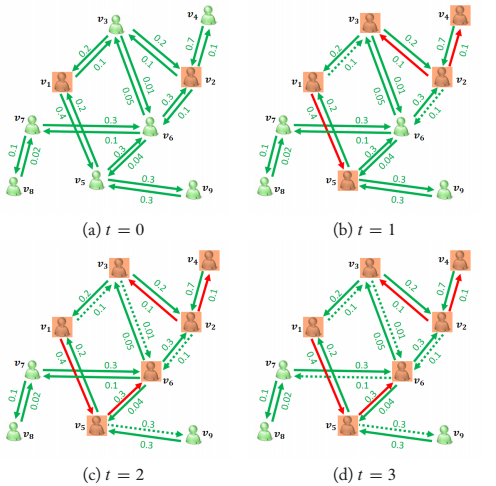
\includegraphics [scale=.5]{picture/Hinh2_1}
				\end{center}
				\caption{Một số ví dụ quá trình lan truyền thông tin trên mô hình IC}
				\label{refhinh2_1}
			\end{figure}
		\end{center}
	Tại thời điểm bắt đầu t=0, hai đỉnh v$_{1}$, v$_{2}$ ở trạng thái {\itshape kích hoạt}. Ở thời điểm t = 1, v$_{1}$ kích hoạt thành công v$_{5}$ nhưng thất bại với v$_{3}$, trong khi đó v$_{2}$ kích hoạt thành công v$_{3}$ và v$_{4}$ nhưng thất bại với v$_{6}$. Tại thời điểm t = 2, v$_{3}$ kích hoạt thất bại v$_{6}$ trong khi v$_{5}$ kích hoạt thành công v$_{6}$ nhưng thất bại với v$_{9}$. Ở bước t = 3, v$_{6}$ kích hoạt thất bại v$_{7}$, đến đây quá trình lan truyền thông tin kết thúc do không có đỉnh nào được kích hoạt thêm.
	
	Mô hình IC phù hợp cho quá trình lan truyền thông tin hoặc virus, đó là các môi trường mà việc tiếp xúc với một nguồn là đủ để một cá nhân được kích hoạt.
	
	\subsection{Mô hình ngưỡng tuyến tính}
	Mô hình IC phù hợp để mô tả sự lan truyền thông tin đơn giản, ở đó một đỉnh có thể được kích hoạt từ một đỉnh duy nhất. Tuy nhiên trong thực tế có nhiều trường hợp một cá nhân cần nhiều sự tác động của các cá nhân khác để thay đổi hành vi của mình. Có thể kể đến các trường hợp như khi người dùng tiếp nhận một thông tin mới, một công nghệ mới, hay một thông tin sai lệch bôi xấu danh dự của các đồng chí lãnh đạo Đảng và Nhà nước, người dùng MXH cần được củng cố tích cực từ nhiều nguồn độc lập trong số bạn bè và người quen của họ trước khi họ thay đổi suy nghĩ của mình, chấp nhận thông tin đó.
	
	Các nhà khoa học đã đề xuất khái niệm {\itshape hành vi ngưỡng} để mô tả các hành vi kiểu như trên. Khi một hàm tổng hợp của các người dùng đã kích hoạt trên mạng đạt đến một ngưỡng nhất định thì  đối tượng sẽ được kích hoạt, xét đến hành vi ngưỡng mà mỗi cá nhân chỉ được kích hoạt khi tiếp nhận ảnh hưởng từ nhiều hơn hai nguồn thông tin.
	
	Mô hình ngưỡng tuyến tính (Linear Threshold – LT) là mô hình khuếch tán ngẫu nhiên được đề xuất bởi Kempe \cite{kemple1}. Trong mô hình LT, mỗi cạnh (u,v) $\in$ [0,1] biểu diễn mức độ ảnh hưởng của đỉnh u đến đỉnh v. Nếu (u,v) $\notin$ E thì w(u,v)=0. Các trọng số này được chuẩn hóa sao cho với mỗi đỉnh v, tổng trọng số tất cả các cạnh đi đến đỉnh v lớn nhất bằng 1, tức là: $\sum$ $_{u}$ w(u,v) $\leq$ 1 %$\in$ N$_{in}$(u) 
	
	Tùy vào đặc tính của từng người dùng tương ứng, mỗi đỉnh v $\in$ V có một giá trị $\theta$$_{v}$ $\in$ [0,1], biểu diễn ngưỡng đỉnh v bị ảnh hưởng bởi các đỉnh kích hoạt hàng xóm. Quá trình lan truyền thông tin trên mô hình LT diễn ra theo bước thời gian rời rạc, tạo ra tập các đỉnh kích hoạt theo quy tắc sau:
	
	- Tại thời điểm t = 0, tập đỉnh ở trạng thái kích hoạt chính là tập nguồn phát thông tin sai lệch S$_{0}$.
	
	- Tại thời điểm t  1, đầu tiên ta gán S$_{t}$ bằng S$_{t-1}$. Sau đó với mỗi đỉnh chưa được kích hoạt v $\in$ V \ S$_{t-1}$, nếu tổng ảnh hưởng từ những đính hàng xóm kích hoạt tới v vượt ngưỡng $\theta$$_{0}$, tức là % $\sum$ $_{u}$ w(u,v) $\geqslant$ $\theta$ $_{0}$ thì đỉnh v được kích hoạt, ta thêm v vào tập S$_{t}$.
	
	- Nếu tại thời điểm t, không có nút nào được kích hoạt thêm nữa, nghĩa là S$_{t}$ = S$_{t-1}$, tập các nút kích hoạt sẽ không còn thay đổi nữa, và quá trình truyền tin kết thúc với tập các nút bị kích hoạt cuối cùng là S$_{t}$.
	
	Sự ngẫu nhiên trong việc lựa chọn ngưỡng $\theta$$_{0}$ từ 0 đến 1 phản ánh sự thiếu thông tin về ngưỡng nội bộ của mỗi cá nhân. Điều này phản ánh khá đúng với thực tế xã hội, bởi vì sự chập nhận thông tin của mỗi người, tại những thời điểm khác nhau là khác nhau, và rất khó để nắm bắt. 
	
	Hình \ref{refhinh2_2} chỉ ra một ví dụ quá trình lan truyền thông tin trên mô hình LT. Các đỉnh màu da cam và màu xanh tương ứng biểu diễn các đỉnh ở trạng thái {\itshape kích hoạt}, và {\itshape không kích hoạt}. Các cạnh liền màu đỏ cùng đến đỉnh v biểu diễn các cạnh này đồng thời cố thử kích hoạt đỉnh v và thành công.
	
	\begin{center}
		\begin{figure}[htp]
			\begin{center}
				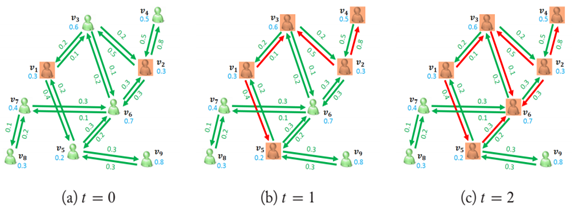
\includegraphics [scale=.75]{picture/Hinh2_2}
			\end{center}
			\caption{Ví dụ quá trình lan truyền trên mô hình LT}
			\label{refhinh2_2}
		\end{figure}
	\end{center}	
	Tại thời điểm t=0, tất cả các đỉnh được khởi tạo ngẫu nhiên ngưỡng $\theta$$_{0}$ $\in$ [0,1], hai đỉnh v$_{1}$ và v$_{2}$ là các đỉnh hạt giống. Ở thời điểm t = 1, v$_{1}$ và v$_{2}$ kích hoạt thành công v$_{3}$, v$_{1}$ cũng phải cách hoạt thành công v$_{5}$ và v$_{2}$ kích hoạt thành công v$_{4}$; tuy nhiên v$_{6}$ lại không kích hoạt thành công vì tổng trọng số các cạnh đi đến v$_{6}$ là 0.3, trong khi ngưỡng kích hoạt của v$_{6}$ 0.7. Tại thười điểm t = 2, các đỉnh hàng xóm đi đến v$_{6}$ là v$_{2}$, v$_{3}$, v$_{5}$ đã được kích hoạt cho nên tổng trọng số các cạnh đi đến là 0.7 đủ để kích hoạt v$_{6}$. Tại bước t = 3, quá trình lan truyền thông tin kết thúc do không có đỉnh nào được kích hoạt thêm.

\section{Một số hướng nghiên cứu liên quan bài toán hạn chế lan truyền thông tin sai lệch trên mạng xã hội}
Tối ưu hóa ảnh hưởng của các đối tượng trên MXH là bài toán liên quan đến lan truyền thông tin trên MXH được nghiên cứu lần đầu tiên bởi Domingos và Richardson, 2001 \cite{pedro}. Sau khi Kempe, 2003 \cite{kemple1} lần đầu tiên xây dựng vấn đề tối ưu hóa ảnh hưởng trên MXH theo cách tối ưu hóa rời rạc, có rất nhiều nghiên cứu liên quan tập trung giải quyết bài toán tối đa hóa ảnh hưởng của thông tin trên mạng xã hội như nghiên cứu của Leskovec, 2007 \cite{leskovec}, Goyal, 2011 \cite{goyal}, Wei Chen, 2014 \cite{chen}.

Bên cạnh vấn đề lan truyền thông tin, lan truyền ảnh hưởng cũng có rất nhiều nghiên cứu tập trung giải quyết bài toán hạn chế thông tin sai lệch lan truyền trên các MXH trực tuyến. Một số nghiên cứu tập trung vào việc nhận dạng thông tin sai lệch và tin đồn (Rumor) dựa trên đặc trưng ngôn ngữ, cấu trúc, thời gian như nghiên cứu của Qazvinian, 2011, \cite{qazvin} và Kwon, 2013, \cite{kwon}.

Một số khác, nghiên cứu vấn đề xác định tập đỉnh là nguồn phát thông tin sai lệch ban đầu. Chẳng hạn, Dung T. Nguyen và các cộng sự, 2012, \cite{nguyen1} đã nghiên cứu bài toán xác định k nguồn phát tán thông tin sai lệch khả nghi nhất từ tập người dùng bị kích hoạt bởi thông tin sai lệch cho trước và chứng minh bài toán thuộc lớp NP-khó xét trên mô hình lan truyền IC, đồng thời nhóm tác giả đã đề xuất hai thuật toán dựa trên cách tiếp cận xếp hạng (Ranking) và cách tiếp cận xấp xỉ đạt tỉ lệ tối ưu 1 - $\dfrac{1}{e}$ - $\varepsilon$

Trong việc hạn chế phát tán thông tin sai lệnh, Zhang \cite{zhang1} để xuất bài toán tìm số nút nhỏ nhất trong khoảng cách $\delta$ (vùng N$_{}$ ()) đối với nguồn phát thông tin sai lệnh để vô hiệu hóa sao cho thông tin sai lệnh đến nút đích r được giới hạn. Bên cạnh đó, một số tác giả đề xuất giải pháp hạn chế sự lan truyền thông tin sai lệch trên mạng xã hội bằng cách chọn ra một số đỉnh ban đầu để tiêm thông tin tốt, từ đó lan truyền những thông tin này trên cùng mạng nhằm thuyết phục những người dùng khác tin theo, trong đó sử dụng các mô hình lan truyền thông tin khác nhau \cite{nguyen9}, \cite{nguyen30}.

Trong việc khử nhiễm đối với nguồn tin sai lệnh, Nguyen \cite{nguyen9} đề xuất bài toán tìm tập người dùng hạt giống sao cho tỷ lệ khử nhiễm sau thời gian T đối với nguồn thông tin sai lệnh I trong mạng là $\beta$ $\in$ (0,1). Tức là khử nhiễm đối với các nguồn phát này sao cho số người dùng được khử nhiễm là $\beta$.|V|. Ceren \cite{ceren} đưa ra bài toán phản bác lại thông tin sai lệnh bằng cách chọn k người dùng để thuyết phục họ nhận thức được các thông tin để phản bác lại, triệt tiêu các thông tin sai lệnh. Trong nghiên cứu này, nhóm tác giả đã xây dựng mô hình Oblivious Independent Campaign, họ chứng minh đây là bài toán NP-Khó và hàm mực tiêu là hàm đơn điệu tăng và submodular.

Liên quan gần nhất đến vấn đề nghiên cứu trong đề tài của nhóm tác giả là công trình nghiên cứu của H. Zhang, 2016 \cite{zhang31}. Trong nghiên cứu của mình, H. Zhang đề xuất hai bài toán: Bài toán phát hiện thông tin sai lệch yêu cầu xác định k vị trí đặt giám sát (Monitor) trên MXH sao cho cực đại hóa xác suất phát hiện thông tin sai lệch và Bài toán đặt giám sát yêu cầu tìm ra tập đỉnh có kích thước nhỏ nhất để đặt giám sát sao cho xác suất thông tin sai lệch kích hoạt thành công đỉnh r nhỏ hơn một ngưỡng cho trước.


\chapter{GIẢI PHÁP NGĂN CHẶN SỰ PHÁT TÁN CỦA THÔNG TIN SAI LỆCH}

Tự do ngôn luận, tự do báo chí là một trong những quyền căn bản của công dân đã được Hiến pháp ghi nhận và đã được Đảng và Nhà nước nhất quán. Tuy nhiên thực tế hiện nay có rất nhiều cá nhân, tổ chức đã và đang lợi dụng các quyền này để xâm phạm lợi ích của Nhà nước và lợi ích chính đáng của công dân. Với sự phát triển mạnh mẽ của Internet và mạng xã hội trực tuyến, việc đăng tải, tuyên truyền các thông tin sai lệch mang tính chất xuyên tạc, chống đối đường lối chính sách của Đảng, pháp luật của Nhà nước, hoạt động của bộ máy chính quyền diễn ra thường xuyên hơn với âm mưu, quy mô và tổ chức ngày càng rộng lớn, chặt chẽ.

Như thường lệ, mỗi khi cơ quan chức năng Việt Nam tiến hành truy tố, xét xử những cá nhân có hành vi vi phạm pháp luật như: Hoạt động nhằm lật đổ chính quyền nhân dân (theo Điều 109 Bộ luật Hình sự năm 2015, sửa đổi bổ sung năm 2017); tuyên truyền chống Nhà nước Cộng hòa XHCN Việt Nam (Điều 117) hay lợi dụng các quyền tự do, dân chủ, xâm phạm lợi ích của Nhà nước, quyền, lợi ích hợp pháp của tổ chức, công dân (Điều 331) thì ngay lập tức một số tổ chức, cá nhân chống đối trong và ngoài nước lại ráo riết tuyên truyền xuyên tạc, chống phá Việt Nam trên lĩnh vực dân chủ, nhân quyền. Những đối tượng này đã lợi dụng quyền tự do ngôn luận để viết và đăng tải các nội dung sai lệch, không có căn cứ, tuyên truyền xuyên tạc đường lối, chính sách của Đảng, pháp luật của Nhà nước, bôi nhọ các cán bộ, Đảng viên làm ảnh hưởng đến uy tín của cơ quan, tổ chức, đi ngược lại với lợi ích quốc gia, dân tộc.

Xuất phát từ những thực tế nêu trên, nhóm tác giả nhận thấy việc nghiên cứu đề ra giải pháp ngăn chặn kịp thời sự lan truyền của thông tin sai lệch trên MXH là một thách thức lớn cần giải quyết kịp thời. Từ thực trạng trên nhóm tác giả đề xuất xây dựng hai bài toán ngăn chặn.

Bài toán đầu tiên với nguồn ngân sách hạn chế, hạn chế bước thời gian lan truyền thông tin, yêu cầu tìm ra $k$ đỉnh có vai trò quan trọng nhất đối với quá trình lan truyền thông tin. Bài toán thứ hai không hạn chế nguồn ngân sách, không hạn chế bước thời gian lan truyền thông tin, yêu cầu tìm tập ít đỉnh nhất đảm bảo số người dùng không bị nhiễm thông tin sai lệch vượt quá một ngưỡng cho trước.

Hai bài toán này đều dựa trên những yêu cầu thực tế, và bản chất của hai bài toán này là các bài toán tối ưu. Ứng với mỗi bài toán, nhóm tác giả đề xuất một thuật toán (giải pháp) tương ứng để giải quyết, đồng thời chứng minh độ tốt về mặt lý thuyết của thuật toán.

Bên cạnh đó, nhóm tác giả còn đưa ra các kết quả thực nghiệm của hai giải pháp đã được đưa ra đối với hai bài toán tương ứng trên dữ liệu đã công bố, từ đó để thấy được hiệu quả của phương pháp nhóm đề xuất về kết quả và thời gian. Dữ liệu đã công bố là các bộ dữ liệu được lấy từ những nguồn uy tín hàng đầu, được các bài báo có chung mục tiêu nghiên cứu khác sử dụng và được các hội nghị, hội thảo thế giới công nhận. Việc thực nghiệm này sau khi đã kiểm chứng độ tốt về mặt lí thuyết cho thấy các giải pháp mà nhóm tác giả đề xuất có hàm lương học thuật cao, khả thi về mặt lý thuyết.

\section{Bài toán 1: Ngăn chặn thông tin sai lệch với ngân sách giới hạn}
Bài toán này được đề xuất và nghiên cứu sau khi xem xét thực tế quá trình lan truyền của một thông tin sai lệch trên mạng xã hội. Thông tin sai lệch luôn bắt đầu từ một số người dùng nhất định (có thể coi như đỉnh “nguồn” phát tán thông tin sai lệch). Những người dùng này thường là những kẻ có tư tưởng lệch lạc, phản động, và thông tin sai lệch thường là những thông tin bị bóp méo, những sai lầm của cán bộ bị thổi phồng, hoặc những lời lẽ bịa đặt vô căn cứ. Từ những người dùng bắt đầu này, thông tin sẽ được biết đến bởi những người xung quanh có liên kết với chúng, thường là những người dùng có quan hệ bạn bè với chúng. Thông tin này ban đầu có thể không tác động tới người dùng xung quanh, tuy nhiên nếu nó xuất hiện thêm nhiều lần từ nhiều nguồn khác nhau thì họ có thể sẽ tiếp nhận thông tin đó, và từ đó trở thành một nguồn phát thông tin sai lệch mới. Nếu mọi việc cứ phát triển thì thông tin này dần dần sẽ lan truyền sang toàn bộ một cộng đồng, hoặc thậm chí là toàn MXH (Quá trình lan truyền này được biểu diễn thông qua mô hình lan truyền được định nghĩa bên dưới). Do đó, cần có phương pháp giúp kiểm soát tình hình, ngăn chặn thông tin sai lệch lan truyền quá rộng, và đây cũng là lí do mà giải pháp này được nghiên cứu và công bố. Giải pháp được thiết kế để có thể chọn một số người dùng đặc biệt. Những người dùng được chọn này sau đó sẽ được các cơ quan chức năng có thẩm quyền tiến hành các phương pháp phù hợp đề ngăn chặn khả năng phát tán thông tin của họ. Từ đó, thông tin sai lệch sẽ không có khả năng truyền thông qua những người dùng này, và dẫn đến khả năng lan truyền sang những người dùng tiếp theo bị cản trở. Giải pháp này đã được chứng minh rằng nó có thể lựa chọn ra các đỉnh hiệu quả nhất để ngăn chặn, do đó vừa đem lại hiệu quả cao mà không hao tốn quá nhiều tài nguyên vào việc ngăn chặn các đỉnh kém hiệu quả khác.
\subsection{Tổng quan bài toán}
Bài toán này được đưa ra nghiên cứu dựa trên những nhận định về việc thông tin lan truyền trên một mạng xã hội trong thực tế từ người dùng này đến người dùng khác có thể được coi như các bước lan truyền thông tin độc lập diễn ra liên tiếp nhau. Nếu ta càng ngăn chặn được sự lan truyền thông tin sai lệch sớm bao nhiêu, thì hậu quả mà thông tin sai lệch để lại sẽ càng được hạn chế bấy nhiêu. Không chỉ thế, các nghiên cứu gần đây cũng đã chỉ ra rằng số các bước lan truyền thường nhỏ, ví dụ như trong \cite{cha23} đã chỉ ra rằng số các bước lan truyền liên tiếp nhau thông thường chỉ nhỏ hơn 4, và trong \cite{lesk16} một bước lan truyền xảy ra thường là giữa hai người dùng có liên kết trực tiếp với nhau.
Giải pháp tập trung vào việc tìm ra tập đỉnh $A$ có tối đa $k$ đỉnh để loại bỏ khỏi đồ thị để có thể tối thiểu hóa tác hại của lan truyền thông tin sai lệch. Những khía cạnh mới mà giải pháp của chúng tôi đề ra so với các công trình trước đó là: quá trình lan truyền được giới hạn trong khoảng $d \geq 1$ bước lan truyền bắt đầu từ nguồn phát tán thông tin sai lệch, và giải pháp được thực hiện trên một mô hình lan truyền xác định bởi thực tế cho thấy thông tin cá nhân của người dùng có thể được thu thập qua khảo sát và các phương pháp khai phá dữ liệu \cite{zaixin}. Cụ thể, giải pháp này của chúng tôi có thể được tóm tắt lại như sau:
\begin{itemize}
	\item Chúng tôi đưa là một mô hình lan truyền thông tin với giới hạn về thời gian lan truyền thông tin, được mở rộng từ mô hình Ngưỡng tuyến tính xác định (Deterministic Linear-Threshold), gọi là mô hình Ngưỡng tuyến tính với bước thời gian rời rạc (Time Constraint Deterministic Linear-Threshold). Sau đó, chúng tôi định nghĩa bài toán Hạn chế sự lây lan của thông tin sai lệch (Limiting the Spread of Epidemics - LSE) với mục tiêu tìm kiếm tập đỉnh $A$ có kích thước tối đa $k$ để loại ra khỏi đồ thị sao cho số đỉnh cứu được là tối đa trong một ràng buộc thời gian. Chúng tôi chỉ ra bài toán này là bài toán NP-Khó.
	\item Với lời giải, chúng tôi đưa ra Thuật toán nhanh và hiệu quả để giới hạn sự lây nhiễm thông tin (Fast And Effective Limiting Epidemics – FLE).
	\item Việc kiểm thử được thực hiện trên các bộ dữ liệu thực tế lấy từ các nguồn đáng tin cậy như Gnutella, Wikipedia Vote, Amazon và Google Web, đồng thời chúng tôi cũng sử dụng một bộ dữ liệu được thu thập trực tiếp trên Facebook Việt Nam. Thuật toán đã được kiểm nghiệm và cho thấy khả năng ưu việt về cả tốc độ lẫn chất lượng lời giải so với các thuật toán phổ biến được dùng. Chi tiết về kiểm nghiệm sẽ được nêu rõ ở chương sau.
\end{itemize}  

\subsection{Mô hình lan truyền thông tin Ngưỡng tuyến tính với bước thời gian rời rạc (Time Constraint Deterministic Linear Threshold - T-DLT).}
Như đã được trình bày ở trên, có hai mô hình phổ biến trong bài toán lan truyền thông tin nói chung là mô hình IC và mô hình LT. Tuy nhiên, ở giải pháp này chúng tôi đề xuất một mở rộng mô hình DLT \cite{zaixin}, vốn cũng là một trường hợp biến thể của mô hình LT, được gọi là T-DLT. Sở dĩ chúng tôi sử dụng mô hình này thay cho mô hình LT và IC bởi với bài toán này, mô hình T-DLT cho phép chúng tôi giảm thiểu tính phức tạp của cơ chế lan truyền, đồng thời vẫn đảm bảo kết quả không bị ảnh hưởng so với hai mô hình điển hình trên. Chi tiết mô hình T-DLT có thể được mô tả như sau:
\begin {itemize}
\item {\itshape Ký pháp đồ thị}: Đặt $G=(V,E,w)$ là biểu diễn của mạng xã hội với tập đỉnh $V$, tập cạnh có hướng $E$, với $|V|=n$ và $|E|=m$. Mỗi đỉnh đại diện cho một người dùng trong mạng xã hội, mỗi cạnh $e=(u,v)$ trong tập $E$ tương ứng đại diện cho mỗi quan hệ giữa người dùng $u$ và người dùng $v$. Chúng tôi ký hiệu đỉnh vào liền kề và đỉnh ra liền kề của đỉnh $u$ lần lượt là $N_{\textup{in}}(u)$ và $N_{\textup{out}}(u)$, $d_{\textup{in}}(u)$ và $d_{\textup{out}}(u)$ lần lượt là bậc vào và bậc ra của đỉnh $u$. Đặt $I \subset V$ là tập các đỉnh bị lây nhiễm ban đầu. Mỗi cạnh có hướng $(u,v)$ sẽ có trọng số $w(u,v)$, tượng trưng cho mức độ ảnh hưởng thông tin của $v$ tới $u$, thỏa mãn $\sum_{u} w(u,v) \leq 1$.

\item {\itshape Trạng thái của đỉnh}: Quá trình phát tán thông tin sai lệch từ tập đỉnh ban đầu $I$ tới các đỉnh còn lại trong mạng xã hội tiến triển theo từng bước thời gian rời rạc $t=1,2,…,d$. Mỗi đỉnh $v \in V$ có hai trạng thái là {\itshape bị lây nhiễm (hay “kích hoạt”)} và {\itshape không bị lây nhiễm (hay “không kích hoạt”)}.

\item {\itshape Ngưỡng lây nhiễm (hay ngưỡng kích hoạt)}: Mỗi đỉnh $v$ sẽ có một ngưỡng lây nhiễm cho trước $\theta_{v} \in [0,1]$. Giá trị này đại diện cho trọng số vào của đỉnh $v$ cần chuyển thành bị lây nhiễm để $v$ trở thành bị lây nhiễm.

\item {\itshape Quá trình lan truyền}: Quá trình lây lan thông tin sai lệch được mô phỏng tuần tự theo từng bước thời gian rời rạc (còn gọi là “vòng”, “bước”) $t=0,1,2,…,d$. Đặt $I_{t}$ là tập các đỉnh bị lây nhiễm sau $t$ bước, quá trình lan truyền được mô phỏng như sau:
\begin {enumerate} [+]
\item Tại bước $t=0$, tất cả các đỉnh trong tập $I$ đều bị lây nhiễm, $I_{0}=I$.

\item Tại bước $t\geq1$, tất cả các đỉnh không bị lây nhiễm $v$ sẽ chuyển thành bị lây nhiễm nếu tổng trọng số các cạnh vào gần kề chạm ngưỡng lây nhiễm của nó, $\sum_{\text{các đỉnh vào gần kề của $u$}} w(u,v) \geq \theta_{v}$.	

\item Một đỉnh bị lây nhiễm sẽ giữ nguyên trạng thái bị lây nhiễm cho tới hết quả trình lan truyền. Qúa trình lan truyền chấm dứt khi $t = d$.
\end {enumerate}
\end {itemize}

Trong mô hình LT, giá trị của ngưỡng $\theta_{v}$ được đặt một cách ngẫu nhiên trong khoảng $[0,1]$ và sẽ được chỉnh sửa dựa vào thông tin có được thêm trong quá trình lan truyền. Do đó, mô hình này thuộc dạng mô hình ngẫu nhiên. Khác với mô hình LT, trong mô hình T-DLT ngưỡng lây nhiễm $\theta_{v}$ được cho trước. Trường hợp này, giá trị ngưỡng có thể được đặt dựa theo các khảo sát thực tế hoặc các phương pháp khai phá dữ liệu.

Mô hình lan truyền T-DLT được chúng tôi lựa chọn để giải quyết bài toán bởi nó phù hợp với quá trình lan truyền thông tin nói chung trong thực tế. Khi một thông tin phát tán từ một nguồn, nó sẽ lan truyền từng bước thông qua những người có liên kết liền kề với nhau. Điều này được mô phỏng rõ dưới cách hoạt động của mô hình lan truyền T-DLT. Mặt khác, mô hình này có thể sử dung các kết quả khai thác dữ liệu từ trước để thiết lập các thông số một cách linh động hơn hẳn so với các mô hình còn lại.

\subsection{Định nghĩa bài toán}
Đối với giải pháp này, việc ngăn chặn thông tin sai lệch được tiến hành bằng cách loại bỏ một số người dùng ra khỏi mạng để thông tin không thể truyền qua được, sao cho phạm vi lan truyền của thông tin là nhỏ nhất có thể. Nếu như coi mạng xã hội là một đồ thị, thì ta có thể hiểu rằng những đỉnh “bị lây nhiễm” là những người dùng đã bị ảnh hưởng bởi thông tin sai lệch và thông tin sai lệch đó có thể truyền từ người dùng này sang những người dùng thân cận, những đỉnh “không bị lây nhiễm” là những đỉnh không bị ảnh hưởng bởi thông tin sai lệch, còn những đỉnh “cứu được” là những đỉnh mà có trạng thái chuyển từ “bị lây nhiễm” sang “không bị lây nhiễm” khi chiến thuật loại bỏ đỉnh được áp dụng. Trong thực tế, việc loại bỏ một người dùng ra khỏi mạng xã hội có thể được thực hiện bằng cách thuyết phục người dùng đó thoát khỏi sự ảnh hưởng của thông tin sai lệch, hoặc ngăn chặn kết nối mạng của người dùng đó, hoặc xóa bỏ tài khoản của người dùng ra khỏi mạng xã hội, v.v… Tuy nhiên, những cách làm này đều là những cách làm yêu cầu có sự phối hợp từ nhiều bên liên quan, do đó nếu tiến hành loại bỏ quá nhiều sẽ dẫn đến chi phí phát sinh về thời gian và vật chất rất lớn, thậm chí sẽ gây ra trường hợp loại bỏ thành công như không kịp thời, khiến thông tin lan truyền quá rộng dẫn đến vô ích. Vì vậy, vấn đề đặt ra là phải làm sao chọn ra được một số lượng $k$ đỉnh nào đó để khi thực hiện chiến thuật loại bỏ, ta có được số đỉnh cứu nhiều nhất. Số lượng $k$ sẽ được tính toán một cách cân đối, cẩn thận nhất về chi phí để không làm mất tác dụng của chiến thuật loại bỏ. Chiến thuật loại bỏ $k$ đỉnh này có thể được mô hình hóa và phát biểu khoa học như sau:  

Kí hiệu $f_{d}(I)$ là tập hợp các đỉnh đã bị lây nhiễm sau $d$ vòng trên đồ thị $G = (V,E)$ trong mô hình T-DLT, $f_{d}(I,A)$ là tập các đỉnh bị lây nhiễm sau khi loại bỏ một tập các đỉnh $A \subseteq V \setminus I$ từ $G$ (số đỉnh bị lây nhiễm trong đồ thị sót lại). Khi đó, số đỉnh cứu được khi loại bỏ tập $A$ là: $h_{d}(A)=| f_{d}(I,\emptyset)|-|f_{d}(I,A)|$.

Trong mô hình T-DLT, ta xây dựng một bài toán tối ưu tổ hợp là: {\itshape Hạn chế sự lây lan của thông tin sai lệch} (Limiting the Spread of Epidemics - LSE), có mục tiêu tìm kiếm một tập đỉnh có kích cỡ tối đa $k$ đỉnh sao cho khi loại bỏ tập đỉnh đó, số đỉnh cứu được sẽ đạt cực đại.  

\begin{define}[Bài toán LSE]
	Cho đồ thị vô hướng $G=(V,E)$ biểu diễn một mạng xã hội trong mô hình T-DLT. Một tập các đỉnh bị lây nhiễm ban đầu $I \subset V$, số vòng lan truyền $d$ và số đỉnh tối đa loại bỏ được là $k > 0$. Tìm một tập $k$ đỉnh  $A \subseteq V \ I$ sao cho khi loại bỏ khỏi mạng thì số đỉnh cứu được sau $d$ vòng là $h_{d}(A)$ đạt cực đại.
\end{define}

Kí hiệu $G_{d} = (V_{d}, E_{d})$ đồ thị con của đồ thị $G=(V, E)$ trong đó $V_{d}$ là tập các đỉnh mà khoảng cách giữa một đỉnh bất kì trong đó với một đỉnh trong tập $I$ tối đa là $d$, và tập $E_{d}$ là tập các cạnh nối giữa các đỉnh thuộc tập $V_{d}$, đồng thời $n_{d} = | V_{d} |$, $m_{d} = | E_{d} |$. Ta thấy rằng sự lan truyền thông tin sai lệch chỉ xảy ra bên trong đồ thị con $G_{d}$. Do đó, để đơn giản hóa, thay vì xét đến tất cả các đỉnh thuộc $G$, ta sẽ chỉ tìm kiếm kết quả trong đồ thị con $G_{d}$.

\subsection{Độ phức tạp của bài toán LSE}
Trong mục này, chúng tôi chỉ ra tính NP-Khó của bài toán LSE bằng phép dẫn đa thức về bài toán LSE từ bài toán Phủ đỉnh (Set Cover). 

\begin{theo}
	LSE là bài toán NP-Khó trong mô hình T-DLT.
\end{theo}

\begin{proof}
	Để chứng minh LSE là bài toán NP-Khó, ta sử dụng phép dẫn đa thức từ bài toán Phủ đỉnh (Set Cover) về bài toán LSE. 
	
	{\bfseries Bài toán Phủ đỉnh (Set Cover - SC):} Cho một số tự nhiên dương $t$, một tập phổ quát $\vartheta = {e_{1}, e_{2}, ... ,e_{M}}$ và tập con $S = {s_{1}, s_{2}, ... , s_{N}}$ ta có thể giả sử rằng $t < M < N$. Bài toán Phủ đỉnh yêu cầu rằng: có tồn tại hay không một lượng $t$ tập con, sao cho hợp của chúng là $\vartheta$.
	
	Bài toán SC đã được chứng minh là bài toán NP-Khó khi kích thước các tập được giới hạn là 3 và mỗi phần tử xuất hiện trong đúng hai tập con. Để giản thể bài toán SC về bài toán LSE, đầu tiên chúng tôi xây dựng một biểu diễn $J_{\text{LSE}}$ của bài toán LSE từ biểu diễn $J_{\text{SC}}$ của bài toán SC. Sau đó chúng tôi chỉ ra rằng nếu $J_{\text{SC}}$ có tồn tại lời giải $S$ kích thước $t$, thì $J_{\text{LSE}}$ có lời giải $A$, $| A | \leq k$ với $h_{d}(A) \geq k + M$ và ngược lại.
	
	{\bfseries Xây dựng phép dẫn:} Cho một biểu diễn $J_{SC} = (\vartheta, S, t)$ của bài toán SC, ta xây dựng biểu diễn $J_{LSE} = (G, I, d, k)$ của bài toán LSE như theo hình \ref{refhinh3_3}
	\begin {itemize}
	\item {\itshape Tập các đỉnh và các cạnh}: với mỗi $S_{i} \in S$, ta xây dựng một đỉnh bị lây nhiễm ban đầu $s_{i} \in I$ và một đỉnh $u_{i}$. Ta có thêm một cạnh có hướng $(s_{i}, u_{i})$. Với mỗi phần tử $e_{j} \in \vartheta$ ta thêm một đỉnh $v_{j}$ và thêm một cạnh có hướng $(u_{i},v_{j})$ với mỗi $u_{i}$. Để thuận tiện, ta đặt $B = {u_{1}, u_{2}, ... , u_{N}}$, $C = {v_{1}, v_{2}, ... , v_{M}}$.
	
	\item {\itshape Ngưỡng lây nhiễm và trọng số}: ta đặt $w(u,v) = 1$,\linebreak $w(u_{i}, v_{i}) = \dfrac{1}{d_{in}(v_{j})}$, $\theta_{u_{i}} = \theta_{v_{i}} = 1$.
	
	\item Sau cùng, ta cho $k = t$, $d = 2$. 		
	
	\begin{figure}[H]
		\begin{center}
			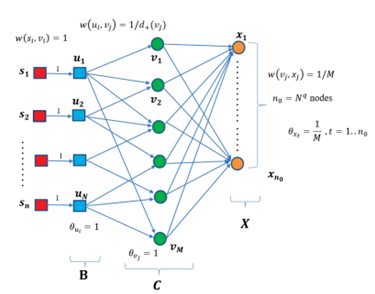
\includegraphics [scale=0.8]{picture/reduce2}
			\caption{Phép dẫn đa thức từ bài toán SC về bài toán LSE.}
			\label{refhinh3_3}
		\end{center}
	\end{figure}
	\end {itemize}
	{\bfseries Phân tích:} Qua bước xây dựng, ta thấy rằng $| f_{d}(I,\emptyset) | = M + N$. Nếu như có đỉnh bất kì $u_{i} \in B$ là đỉnh kề vào và $v_{j} \in C$ là đỉnh chưa bị lây nhiễm thì: 
	\begin{center}
		$\sum_{\text{Các đỉnh hàng xóm tới đã bị lây nhiễm $u$}} w(u, v_{j}) \leq 1 - \dfrac{1}{d_{in}(v_{j})} < 1 = \theta_{v_{j}}$.
	\end{center}
	
	Do đó $v_{j}$ lầ đỉnh không bị lây nhiễm. Nếu không, các đỉnh trong $C$ là các đỉnh không bị lây nhiễm.
	
	($\rightarrow$) Giả sử $S'$ là lời giải của biểu diễn $J_{\text{SC}}$, có nghĩa là $| S' | = t = k$ và nó phủ $t$ phần tử của $\vartheta$. Nếu ta chọn tập $A$ chứa đỉnh $u_{i}$ tương ứng với $S_{i} \in S'$, với mọi đỉnh $v_{i} \in B$ kề với ít nhất một đỉnh trong $A$. Bằng bước phân tích trên, mọi đỉnh trong $C$ là đỉnh không bị lây nhiễm. Ta có $h_{d}(A) = t + M = k + M$.
	
	($\leftarrow$) Ngược lại, nếu $J_{\text{LSE}}$ có lời giải $A$, $|A| \leq k$ với $h_{d}(I, A) \geq k + M$. Nếu $A$ chứa $t_{1} (1 \leq t_{1} \leq k)$ đỉnh trong $C$, $h_{d}(I, A) \leq k - t_{1} + M < k + M$. Do đó $A$ không chứa bất kì đỉnh nào thuộc $C$. Ở đây, $A \subset B$. Kết hợp với $h_{d}(I, A) \geq k + M$, mọi đỉnh thuộc $C$ là đỉnh không bị lây nhiễm. Do đó, mọi đỉnh $u_{i} \in A$ kề ít nhất với một đỉnh thuộc $C$. Vì vậy, qua bước xây dựng ta thấy rằng, $S' = \{ S_{i} | u_{i} \in A \}$ là lời giải cho bài toán $J_{\text{SC}}$. Định lý được chứng minh.
\end{proof}

\subsection{Thuật toán đề xuất}
Trong phần này, chúng tôi thiết kế một thuật toán heuristics có độ phức tạp thấp và kết quả rất khả quan. Tên gọi của thuật toán là Thuật toán nhanh và hiệu quả để giới hạn sự lây nhiễm thông tin(Fast And Effective Limiting Epidemics – FLE). 
Trước khi bắt đầu, chúng tôi có định nghĩa một vài kí hiệu sẽ được sử dụng trong quá trình đề xuất thuật toán:
\begin {itemize}
\item $t(u)$: vòng nhỏ nhất sao cho đỉnh $u$ chuyển từ đỉnh không bị lây nhiễm sang đỉnh bị lây nhiễm.

\item $a_{\text{in}}(u) = \sum_{I_{t(u) - 1} \bigcap N_{in}(u)} w(u,v):$ tổng trọng số các cạnh vào từ các đỉnh vào hàng xóm đã bị lây nhiễm trước vòng $t(u)$.

\item $\alpha(u) = \sum_{v \in U^{d}_{i=t(u)+1}} I_{i} \bigcap N(u)$ $w(u,v), i = t(u) + 1, ... , d$: tổng trọng số các cạnh ra từ $u$ tới các đỉnh bị lây nhiễm $v$ tại vòng $i$.

\item $\beta(u)$: số lượng các đỉnh ra cứu được, sao cho chúng chuyển từ bị lây nhiễm thành không bị lây nhiễm sau khi loại bỏ đỉnh $u$ ra khỏi đồ thị.
\end {itemize}
\begin{algorithm}[H]
	\caption{Fast Limit Epidemics (FLE) algorithm.}
	\label{alg:Algo1}
	%\SetAlgoNlRelativeSize{0}
	\KwData{Graph $G=(V,E,\emptyset)$, set of initial infected nodes $I$, propagation hop $d$.}
	\KwResult{Set of nodes $A$}
	$S \gets \emptyset$; 
	\\
	Calculate $G' \gets G_{d}(I); U \gets V_{d}$
	\\
	\For {$i=1$ to $k$}
	{
		Calculate $\alpha(u)$, $\beta(u)$ on $G'$ (Algorithm 3)
		\\
		$u_{\text{max}} \gets 0$
		\\
		\eIf {$\beta(v)=0, \forall u \in U$}
		{
			$u_{\text{max}} \gets \text{arg max}_{v \in U}\alpha(v)$
		}
		{
			$u_{\text{max}} \gets \text{arg max}_{v \in U}\beta(v)$
		}
		$S \gets S \cup \{u_{\text{max}}\}$
		\\
		$U \gets U \setminus \{u_{\text{max}}\}$
		\\
		Remove $u_{\text{max}}$ and all edges that adjacent with $u_{\text{max}}$ from $G'$
	}
	\Return $S$
\end{algorithm}

Một cách trực quan, số lượng gia tăng các đỉnh được cứu $\delta(A, u)$ có thể xấp xỉ theo $\beta(u)$. Bên cạnh đó, để tăng cường tính hiệu quả của thuật toán đề xuất, chúng tôi kết hợp $\alpha(u)$ và $\beta(u)$ để tính toán khả năng lan truyền tin sai lệch của đỉnh $u$. Ý tưởng chính của thuật toán là chọn ra các đỉnh một cách lần lượt theo đánh giá của hai hàm $\alpha$ và $\beta$. Ban đầu, chúng tôi khởi tạo tập đỉnh được chọn $A=\emptyset$ và đặt tập các đỉnh được xét chọn $U$ bằng với $V_{d}$. Trong mỗi bước, chúng tôi chọn ra đỉnh có trị số $\beta(u)$ lớn nhất trong đồ thị còn lại. Trường hợp tất cả các đỉnh đều có giá trị $\beta(u)$ là 0, chúng tôi chọn đỉnh có giá trị $\alpha(u)$ cực đại. Chi tiết thuật toán được mô tả trong Thuật toán \ref{alg:Algo1}.

Khó khăn trong thuật toán chủ yếu đến từ bước tính toán các hàm $\alpha$ và $\beta$. Để giải quyết việc này, chúng tôi bắt đầu với ý tưởng tìm kiếm theo chiều rộng (Breath First Search - BFS) để tính toán $f_{d}(I)$ và dần dần cập nhật hàm $\alpha_{\text{in}}()$. Sau đó, chúng tôi sử dụng nó để tính toán các hàm  $\alpha()$ và $\beta()$ theo định nghĩa của chúng. Chi tiết thuật toán được thể hiện trong Thuật toán \ref{alg:Algo2} và Thuật toán \ref{alg:Algo3}.
\begin{algorithm}[hpt]
	\caption{Calculate $f_{d}(I), a_{\text{in}}(), t()$}
	\label{alg:Algo2}
	\KwData{Graph $G=(V,E,\emptyset)$, set of infected nodes $I$, propagation hop $d$.}
	\KwResult{$f_{d}(I), a_{\text{in}}(u), t(u), \forall u \in G$.}
	\ForEach {$u$ \textbf{in} $G$}
	{
		$t(u) \gets +\infty; a_{\text{in}}(u) \gets 0; \alpha(u) \gets 0; \beta(u) \gets 0$
	}
	\ForEach {$s$ \textbf{in} $I$}
	{
		$t(s) \gets 0$
	} 
	Queue $Q \gets \emptyset$
	\\
	\While{$Q \neq \emptyset$}
	{
		$u \gets Q.pop()$
		\\
		$f_{d}(I) \gets u$
		\\
		\If{$t(u)<d$}
		{
			\ForEach{$v \in N_{\text{out}}(u)$}
			{
				\If{$t(u)<t(v)$}
				{
					$a_{\text{in}}(v)=a_{\text{in}}(v)+w(u,v)$
					\\
					\If{$a_{\text{in}}(v) \geq \theta_{v}$ \textbf{and} $t(u)+1<t(v)$}
					{
						$t(v) \gets t(u)+1$
						\\
						$Q,push(v)$
					}
				}
			}
		}	
	}
\end{algorithm}

\begin{algorithm}[hpt]
	\caption{Calculate $\alpha()$ and $\beta()$}
	\label{alg:Algo3}
	\KwData{Graph $G=(V,E,\emptyset)$, set of infected nodes $I$, propagation hop $d$, $f_{d}(I), a_{\text{in}}(), t()$.}
	\KwResult{$\alpha(u), \beta(u), \forall u \in G$.}
	\ForEach{$u$ \textbf{in} $f_{d}(I)$}
	{
		$\alpha(u) \gets 0; \beta(u) \gets 0$
		\\
		\ForEach{$v$ \textbf{in} $N_{\text{out}}(u) \cap f_{d}(I)$}
		{
			\If{$t(u)<t(v)$}
			{
				$\alpha(u) \gets \alpha(u)+w(u,v)$
				\\
				\If{$a_{\text{in}}(v)-w(u,v)<\theta_{v}$}
				{
					$\beta(u) \gets \beta(u)+1$
				}
			}
		}
	}
\end{algorithm}

Để đánh giá độ phức tạp của thuật toán này, chúng ta cần đánh giá trước độ phức tạp của thuật toán. Ta dễ thấy rằng việc tính  toán $f_{d}(I)$ (Thuật toán \ref{alg:Algo2}, dòng 7 - 22) có cách thức hoạt đông giống BFS. Do đó, độ phức tạp của nó là $O(m_{d} + n_{d})$. Với bước tính toán $\alpha(u)$ và $\beta(u)$ (Thuật toán \ref{alg:Algo3}, dòng 1 - 11), ta thấy độ phức tạp của nó là $O(m_{d} + n_{d})$. Do đó, độ phức tạp chung của thuật toán là $O(m_{d} + n_{d})$. 

\subsection{Kết quả thực nghiệm với dữ liệu đã công bố}

Trong phần này, chúng tôi thực nghiệm thuật toán đối với dữ liệu sẵn có trên một số mạng xã hội trực tuyến để kiểm chứng tính hiệu quả của thuật toán khi so sánh nó với các thuật toán cơ sở được sử dụng trong các bài toán lan truyền thông tin \cite{nguyen30}, \cite{kemple1}, \cite{zhang32}. Chúng tôi so sánh đánh gia trên ba yêu tố chính: chất lượng lời giải, tính mở rộng, tác động của số vòng lan truyền $d$ trên một vài các mạng xã hội trực tuyến thực tiễn. Các thuật toán cơ sở sẽ sử dụng bao gồm:
\begin{itemize}
	\item Random: Thuật toán chọn ngẫu nhiên $k$ đỉnh trong $N_{d}(S)$.
	
	\item Maxdegree (Maxdeg): Thuật toán heuristic chọn lần lượt các đỉnh có bậc cao nhất trong tập $V_{d}$ cho đến khi đủ $k$ đỉnh.
	
	\item Greedy: Thuật toán heuristic chọn lần lượt $k$ đỉnh, trong mỗi lần chọn sẽ chọn ra đỉnh sao cho khi loại bỏ đỉnh đó sẽ cứu được nhiều đỉnh nhất có thể.
\end{itemize}

Chúng tôi thực nghiệm sử dụng một hệ thống máy có cấu hình sau: Intel(R) Core(TM) i5-6200U CPU @ 2.30 GHz (up to 2.40 GHz), bộ nhớ RAM 4GB, ngôn ngữ lập trình Python 2.7.

\subsubsection{Dữ liêu:}

Chúng tôi thực nghiệm thuật toán trên nhiều bộ dữ liệu thực tế khác nhau. Bên cạnh việc lựa chọn các bộ dữ liệu để đảm bảo sự đa dạng về kích thước, chúng tôi cũng lựa chọn nhiều miền dữ liệu khác nhau, bảng \ref{tab:Table1} thể hiện các bộ dữ liệu nhóm tác giả sử dụng.
\begin{table}
	\centering
	\begin{tabular}{|c|c|c|c|c|}
		\hline 
		Mạng & Số đỉnh & Số cạnh & Loại & Bậc trung bình \\ 
		\hline 
		Gnutella & 6,301 & 20,777 & Có hướng & 3.29 \\ 
		\hline 
		Wikipedia vote & 7,115 & 103,689 & Có hướng & 14.57 \\ 
		\hline 
		Amazon & 262,111 & 1,234,877 & Có hướng & 4.71 \\ 
		\hline 
		Google web & 875,713 & 5,105,039 & Có hướng & 5.83 \\ 
		\hline 
	\end{tabular} 
	\caption{Các bộ dữ liệu}
	\label{tab:Table1}
\end{table}

\subsubsection{Thiết lập tham số}
Chúng tôi sử dụng các thiết lập tham số dưới đây cho việc đánh giá thực nghiệm:

\begin{itemize}
	\item Trọng số của cạnh: $w(u,v)=\frac{1}{d_{\text{in}}(v)}$, với $d_{\text{in}}(v)$ là bậc vào của đỉnh $v$ \cite{kemple1} \cite{chen10LT} \cite{khali} \cite{amit21}.
	\item Ngưỡng lây nhiễm: chúng tôi lựa chọn ngưỡng lây nhiễm trong tập \\ $\{0.1, 0.2, 0.3, 0.4, 0.5, 0.6, 0.7, 0.8, 0.9\}$.
	\item Số vòng lây nhiễm: chúng tôi lựa chọn số vòng lây nhiễm $d = 2, 3, 4, 5$ dựa theo một nghiên cứu có trước \cite{cha23}.
	\item Số đỉnh bị nhiễm ban đầu: trong mọi bộ dữ liệu, chúng tôi lấy $1\%$ số đỉnh làm tập đỉnh bị lây nhiễm ban đầu. 
\end{itemize}

\subsubsection{Các thuật toán sử dụng}
Chúng tôi sử dụng các thuật toán sau đây cho việc đánh giá thực nghiệm cùng với thuật toán FLE, các thuật toán này đều là các thuật toán được sử dụng trong các nghiên cứu liên quan đã có trước:

\begin{itemize}
	\item {\itshape Random}: Thuật toán lựa chọn ngẫu nhiên $k$ đỉnh trong đồ thị mạng xã hội để loại bỏ.
	\item {\itshape Greedy}: Thuật toán thực hiện $k$ lần, mỗi lần chạy thuật toán sẽ thử loại bỏ lần lượt từng đỉnh ra khỏi đồ thị và đánh giá số lượng đỉnh cứu được tuong ứng, qua đó lựa chọn ra đỉnh loại đi mà cứu được nhiều đỉnh nhất để loại bỏ.
	\item {\itshape MaxDegree}: Thuật toán thực hiện $k$ lần, mỗi lần chọn thuật toán sẽ chọn ra đỉnh có bậc lớn nhất để loại nó ra khỏi đồ thị. 
\end{itemize} 

\subsubsection{Kết quả thực nghiệm}

- {\itshape Kết quả lời giải:}

Chúng tôi đo đạc hiệu suất của thuật toán trong ba trường hợp: (1) giá trị $k$ thay đổi từ $10$ đến $100$, $d=5$, $\theta=0.5$ (hình \ref{fig:FLE_k}); (2) ngưỡng $\theta$ thay đổi, $d$ và $k$ giữ nguyên giá trị $50$ (hình \ref{fig:FLE_theta}); (3) giá trị vòng lây nhiêm $d$ thay đổi, $\theta$ và $k$ không đổi (hình \ref{fig:FLE_d}). Trong mọi trường hợp, FLE và Greedy cho kết quả tốt hơn so với các thuật toán còn lại, cụ thể là số lượng đỉnh cứu được nhiều hơn $48.5$ lần so với thuật toán MaxDegree và Random trong hai bộ dữ liệu Gnutella và Wiki Vote. Khi so sánh Greedy và FLE, chúng tôi thấy Greedy có hiệu suất tốt hơn từ $1.02$ đến $1.05$ lần so với FLE trong bộ dữ liệu mạng Gnutella. Tuy nhiên, khoảng cách này bị thu hẹp lại khi $\theta$ và $k$ tăng. Đặc biệt khi $k \geq 50$ và $\theta \geq 0.4$, hiệu suất của hai thuật toán là tương đương nhau. Hình \ref{fig:FLE_k}, \ref{fig:FLE_theta}, \ref{fig:FLE_d} cho thấy Greedy và FLE có hiệu suất tương đương nhau trong bộ dữ liệu mạng Wiki Vote. Trong khi Greedy không thể chạy trong thời gian cho phép trên bộ Amazon và Google Web, FLE vẫn có thể đưa ra kết quả tốt hơn nhiều so với hai thuật toán còn lại.

- {\itshape Kết quả thời gian:}

Thời gian chạy của thuật toán cũng được mô tả trong hình \ref{fig:FLE_k}, \ref{fig:FLE_theta}, \ref{fig:FLE_d}. Đúng như dự đoán, thời gian chạy của Greedy là cực kỳ cao so với các thuật toán còn lại, chiếm $4.5$ phút cho bộ dữ liệu Gnutella và $20.2$ phút cho mạng Wiki Vote. Thuật toán FLE nhanh hơn từ $4820$ đến $6789$ lần so với Greedy trong mạng Gnutella và nhanh hơn từ $5839$ đến $14490$ lần so với Greedy trong mạng Wiki Vote. Điều này xảy ra do Greedy có độ phức tạp thuật toán lớn $O(n_{d}k(m_{d}+n_{d}))$, trong khi FLE chỉ có độ phức tạp nhỏ hơn nhiều $O(k(m_{d}+n_{d}))$. Trong bộ dữ liệu Amazon và Google Web, Greedy không thể tìm thấy lời giải trong vòng $12$ tiếng và bị buộc dừng chạy, trong khi FLE chỉ mất $0.45$ giây và $7.8$ giây tương ứng với mỗi bộ dữ liệu trên. Điều này cho thấy FLE vẫn chạy tốt ngay cả với các bộ dữ liệu lớn.

- {\itshape Ảnh hưởng của tham số $d$:}

Chúng tôi khám phá ảnh hưởng của tham số $d$ đối với các thuật toán khác nhau. Cho $d$ thay đổi từ $2$ đến $5$ trong mạng Gnutella, kết quả được thể hiện trong hình \ref{fig:FLE_d}. Với Greedy và FLE, số đỉnh cứu được tăng khi giá trị $d$ tăng. Đăc biệt, số đỉnh cứu được tăng mạnh với $d=2,3$ và tăng ít hơn với $d=4,5$. Điều này chứng tỏ để ngăn chặn lây lan, ta phải loại bỏ đỉnh càng sớm càng tốt.


- {\itshape Ảnh hưởng của tham số $\theta$:}

Chúng tôi cũng xem xét ảnh hưởng của tham số $\theta$ đối với các thuật toán bằng cách cho $\theta$ thay đổi trong khi giữ nguyên $d$ và $k$. Chúng tôi lựa chọn giá trị $d=5$, $k=50$. Đối với mạng Amazon và Google Web, số đỉnh cứu được sẽ giảm nếu giá trị $\theta$ giảm. Đối với mạng Gnutella và Wiki Vote, số đỉnh cứu được tăng khi $\theta$ tăng từ $0.1$ đến $0.3$ và giảm khi $\theta$ tăng từ $0.3$ đến $0.9$. Tổng quát lại, ta có thể thấy rằng thự tế việc giá trị $\theta$ càng cao sẽ làm quá trình lây làn gặp khó khăn. Từ hình \ref{fig:FLE_theta}, ta thấy Greedy và FLE cho kết quả tốt hơn nhiều so với hai thuật toán còn lại. Điều này một lần nữa cho thấy tính ưu việt của thuật toán FLE.

\begin{figure}[H]
	\begin{tabular}{lll}
		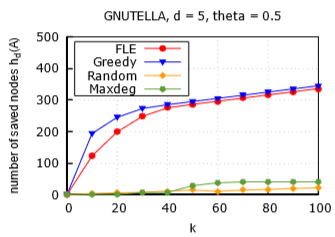
\includegraphics[height = 4.4cm]{picture/FLE/gnu_res} &
		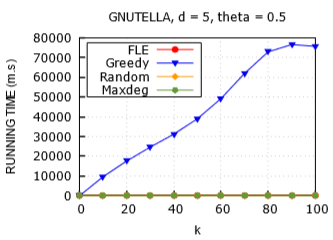
\includegraphics[height = 4.4cm]{picture/FLE/gnu_time} 
		\\
		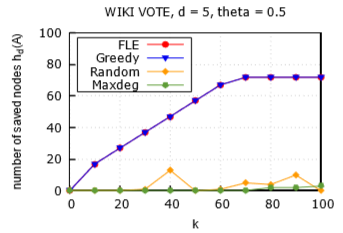
\includegraphics[height = 4.4cm]{picture/FLE/wiki_res} &
		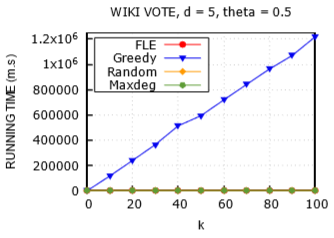
\includegraphics[height = 4.4cm]{picture/FLE/wiki_time} 
		\\
		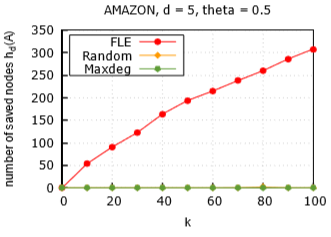
\includegraphics[height = 4.4cm]{picture/FLE/amazon_res} &
		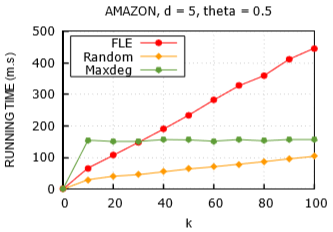
\includegraphics[height = 4.4cm]{picture/FLE/amazon_time} 
		\\
		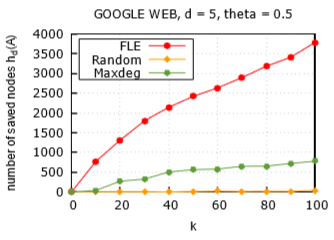
\includegraphics[height = 4.4cm]{picture/FLE/google_res} &
		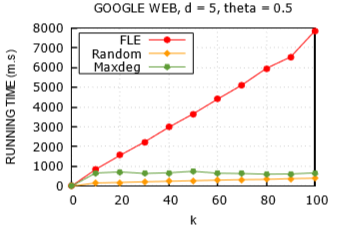
\includegraphics[height = 4.4cm]{picture/FLE/google_time} 
	\end{tabular}
	\caption{So sách chất lượng lời giải và thời gian chạy của các thuật toán khi $k$ thay đổi, $d=5$, $\theta=0.5$.} 
	\label{fig:FLE_k}   
\end{figure}

\begin{figure}[H]
	\begin{tabular}{lll}
		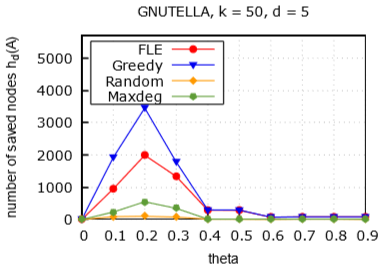
\includegraphics[height = 4.4cm]{picture/FLE/gnu_res_theta} &
		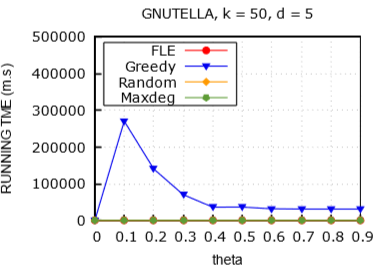
\includegraphics[height = 4.4cm]{picture/FLE/gnu_time_theta} 
		\\
		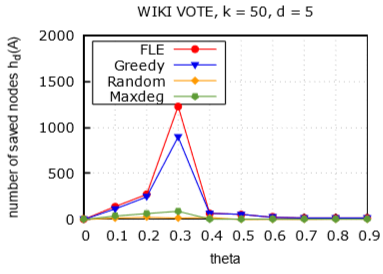
\includegraphics[height = 4.4cm]{picture/FLE/wiki_res_theta} &
		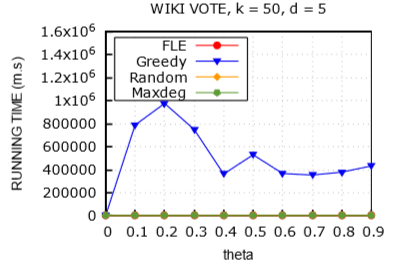
\includegraphics[height = 4.4cm]{picture/FLE/wiki_time_theta} 
		\\
		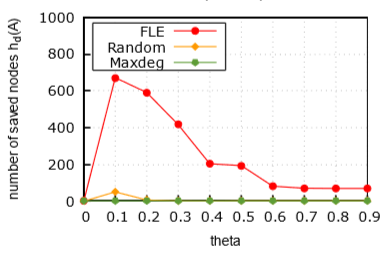
\includegraphics[height = 4.4cm]{picture/FLE/amazon_res_theta} &
		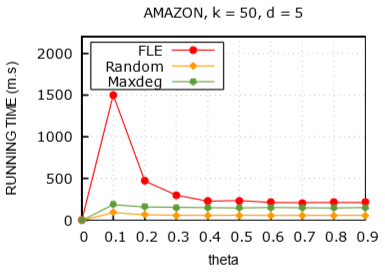
\includegraphics[height = 4.4cm]{picture/FLE/amazon_time_theta} 
		\\
		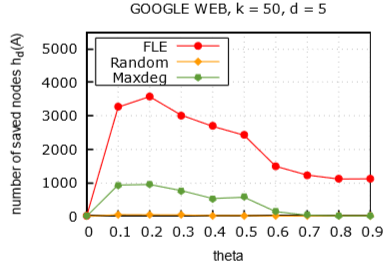
\includegraphics[height = 4.4cm]{picture/FLE/google_res_theta} &
		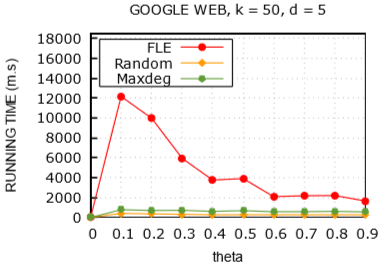
\includegraphics[height = 4.4cm]{picture/FLE/google_time_theta} 
	\end{tabular}
	\caption{So sách chất lượng lời giải và thời gian chạy của các thuật toán khi $\theta$ thay đổi, $d=5$, $k=50$.} 
	\label{fig:FLE_theta}   
\end{figure} 

\begin{figure}[H]
	\begin{tabular}{lll}
		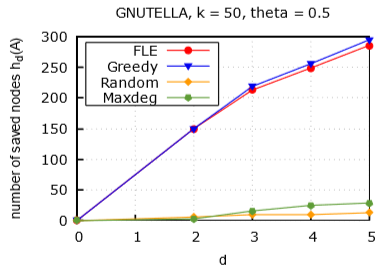
\includegraphics[height = 4.4cm]{picture/FLE/gnu_res_d} &
		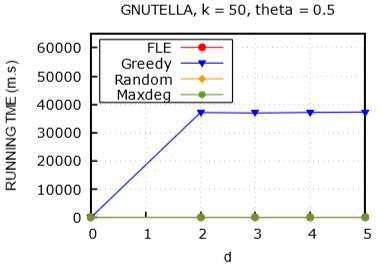
\includegraphics[height = 4.4cm]{picture/FLE/gnu_time_d}
	\end{tabular}
	\caption{So sách chất lượng lời giải và thời gian chạy của các thuật toán khi $d$ thay đổi, $\theta=0.5$, $k=50$ trong mạng Gnutella.} 
	\label{fig:FLE_d}   
\end{figure} 







\section{Bài toán 2: Tìm chi phí nhỏ nhất để ngăn chặn thông tin sai lệch}

Với cách tiếp cận như cách Twitter đã làm năm 2016 là loại bỏ 125.000 tài khoản được nghi ngờ có liên quan đến các hoạt động khủng bố, hay cách tiếp cận như Facebook đã xóa 30.000 tài khoản giả mạo lan truyền các tin đồn trước cuộc bầu cử tổng thống Pháp năm 2017, bài toán Targeted Misinformation Blocking được đưa ra nghiên cứu nhằm mục đích tìm giải pháp xác định được những tài khoản cần loại bỏ khỏi mạng để hạn chế sự phát tán thông tin sai lệch một cách tối ưu nhất.

\subsection{Tổng quan bài toán}
Nguồn phát tán thông tin sai lệch có thể được phát hiện qua các phương pháp khảo sát, khai phá dữ liệu \cite{qazvin, kwon} và được biểu diễn dưới dạng là tập hợp các đỉnh. Theo các nghiên cứu mới đây \cite{khali, tong, pra}, chiến thuật hiệu quả trong việc ngăn chặn phát tán thông tin sai lệch là xóa bỏ đỉnh hoặc cạnh có vai trò quan trọng trong việc lan truyền thông tin sai lệch. Song tính khả thi của các nghiên cứu trước đây lại bị hạn chế bởi một số khía cạnh sau. Thứ nhất họ tập trung vào việc ngăn ngừa thông tin sai lệch bằng nguồn ngân sách hạn chế. Điều này rõ ràng là không thực tế bởi chúng ta khó có thể xác định được bao nhiêu ngân sách cho đủ để ngăn chặn sự lây lan sao cho hiệu quả. Thứ hai, để đảm bảo độ tin cậy của mạng xã hội, chúng ta cần có một biện pháp "khử nhiễm" thông tin sai lệch với một ngưỡng cho trước, như tỉ lệ giữa người dùng bị nhiễm và người dùng được khử nhiễm. Do đó bài toán này được đưa ra với tính thực tế cao hơn đó là: dùng ít ngân sách nhất sao cho số lượng người dùng được khử nhiễm lớn hơn một ngưỡng cho trước. Giải pháp đưa ra nhằm tìm một tập đỉnh có ít phần tử nhất để loại bỏ khỏi đồ thị để sao cho nguồn phát tán thông tin sai lêch không thể lan truyền tới được ít nhất ngưỡng $\gamma$ đỉnh yêu cầu. Tổng quan về giải pháp của chúng tôi được tóm lược như sau:
\begin{itemize}
	\item Đầu tiên chúng tôi định nghĩa bài toán Xác định và ngăn chặn thông tin sai lệch (Targeted Misinformation Blocking - TMB). Và sau đó chứng minh bài toán TMB thuộc lớp bài toán $\#P-\text{khó}$.
	\item Với hàm mục tiêu chúng tôi chứng minh nó là hàm submodular và monotone. Trên cơ sở đó, đề xuất một thuật toán tham lam với với tỉ lệ $1+ln(\gamma/\epsilon)$. Song do những hạn chế của thuật toán tham lam, chúng tôi xây dựng thuật toán Scalable $\mathsf{TMB}$ for LT model Algorithm ($\mathsf{STMB}$) để giải quyết cho bài toán TMB với những dữ liệu lớn hơn. 
	\item Việc thực nghiệm được triển khai trên các bộ dữ liệu đã công bố thu thập từ nguồn uy tín và một bộ dữ liệu được chúng tôi thu thập từ mạng xã hội Facebook. 
\end{itemize}

\subsection{Mô hình lan truyền thông tin Ngưỡng tuyến tính Linear Threshold}
Bài toán này sử dụng mô hình lan truyền thông tin Ngưỡng tuyến tính Linear Threshold. Mô hình lan truyền này là mô hình phổ biến, thường được sử dụng trong các nghiên cứu về mạng xã hội. Chi tiết về mô hình LT đã được trình bày trong chương \ref{chap:2}, ta có thể tóm gọn quá trình lan truyền thông tin trên mô hình LT như sau:

Trong mô hình LT, mỗi đỉnh $v \in V$, có hai trạng thái active và inactive. Quá trình lan truyền trên mô hình LT được diễn tả như sau: Đầu tiên, mỗi đỉnh v được gán một trọng số ngẫu nhiên $\theta_{v} \in [0,1]$ thể hiện giá trị active của đỉnh kề u phải đạt được để có thể active v. Tiếp đến quá trình lan truyền diễn ra trong các vòng t = 1,2,3… như sau: 		
\begin {itemize}
\item Ở vòng 1, tất cả các đỉnh $s_{i} \in S$ ở trạng thái active và các đỉnh còn lại ở trạng thái inactive.

\item Ở vòng t > 1, một đỉnh v ở trạng thái inactive được active nếu thỏa mãn điều kiện $$\sum_{\mbox{ $u \in N_{in}(v) $ và  u  là active}} w(u, v)\geq \theta_v$$

\item Khi một đỉnh ở trạng thái active thì sẽ luôn duy trì trạng thái đó trong suốt quá trình lan truyền thông tin. Quá trình lan truyền kết thúc khi không có đỉnh nào được active thêm.	
\end {itemize}

\subsection{Định nghĩa bài toán}
Kí hiệu $G = (V, E, w)$ là một đồ thị có hướng biểu diễn cho một mạng xã hội trên mô hình $LT$ với $V$ biểu diễn tập người dùng, $E$ biểu diễn mối quan hệ giữa các cặp người người dùng, $w$ là tập trọng số của các cạnh biểu diễn tần số tương tác giữa các người dùng. Gọi $N_{out}(v)$ và $N_{in}(v)$ lần lượt là tập đỉnh đi ra từ $v$ và đi vào $v$. Mỗi cạnh có hướng $(u,v) \in E$ được gán một trọng số $w(u,v) \in [0,1]$ đảm bảo điều kiện $\sum_{u \in N_{in}(v)} \leq 1$.

Đưa ra một tập nguồn $S = {s_{1}, s_{2}, ... , s_{n}}$, $s_{i} \in V$ là tập tiềm năng phát tán thông tin sai lệch (tương tự như tập hạt giống trong bài IM \cite{kemple2}).

Kí hiệu $\sigma_{S}(G)$ là ảnh hưởng lan truyền của tập S trên đồ thị G dưới mô hình LT hay là số lượng đỉnh được active bởi nguồn S. Theo nghiên cứu của Kempe và các cộng sự \cite{kemple1} đã chỉ ra rằng mô hình LT là tương đương với khả năng tiếp cận trong một đồ thị ngẫu nhiên g, thường được gọi là đồ thị live-edge hoặc đồ thị mẫu. Trên mô hình LT, đồ thị live-edge được xây dựng như sau:
\begin {itemize}
\item Với mỗi v $\in$ V, chọn tối đa một cạnh đi vào nó một cách ngẫu nhiên, xác suất cạnh (u, v) được chọn là w(u, v).

\item Xác suất không có cạnh nào được chọn là 1 - $\sum_{u \in N_{in}(v)} w(u,v)$.
\end {itemize}

Cạnh được chọn gọi là cạnh sống (live-edge) và tất cả các cạnh khác gọi là cạnh bị chặn (blocked-edge). Chúng ta có xác suất tạo ra một đồ thị live-egde g từ G là:
\begin{align}
\Pr[g|G]=\prod_{v \in V}{p(v,g,G)}
\end{align}
với
\begin{equation}
p(v, g, G)= \left\{ \begin{array}{ll}
w(u, v), & \mbox{Nếu $\exists u: (u, v) \in E_g$}\\
1-\sum_{u:(u, v) \in E}{w(u, v)}, & \mbox{Trường hợp khác}\\
\end{array} \right.
\end{equation}

Ảnh hưởng lan truyền của nguồn S khi xóa bỏ các đỉnh trong tập A trên đồ thị G[V$\backslash$A] kí hiệu là $\sigma_{S}(G \backslash A)$. Với A = $\emptyset$, trong \cite{kemple1} đã chỉ ra ảnh hưởng lan truyền của tập nguồn S trên G được tính bởi công thức:
\begin{align}
\sigma_S(G)=\sum_{g \in X_G}{\Pr[g|G]|R(g, S)|}
\label{inf_cal}
\end{align}
trong đó $R(g, S)$ là tập các đỉnh đến được từ S trên g và $X_G$ là tập tất cả các đồ thị live-edge được tạo ra từ G. Đặc biệt, ảnh hưởng lan truyền của tập $S$ có thể được tính bằng đường đi đơn bắt đầu từ $u \in S$ theo công thức: 
\begin{align}
\sigma_{S}(G)=\sum_{x \in \mathsf{P}(G, S)} \prod_{e \in x}w(e)
\label{inf_path}
\end{align} 				
với $\mathsf{P}(G, S)$ là tập tất cả các đường đi đơn từ $s \in S$ tới bất kỳ đỉnh $v \in G \setminus \{S \cup \{s\} \} $ trên đồ thị $G$.		

\textbf{Phát biểu bài toán (Bài toán TMB):} Gọi $G(V,E,w)$ là một đồ thị có hướng biểu diễn một mạng xã hội. Đưa ra một tập nguồn $S = {s_{1}, s_{2}, ... , s_{k}}, S \in V$ là tập tiềm năng phát tán thông tin sai lệch và một số nguyên $\gamma \leq | V |$ thể hiện cho số lượng người dùng tối thiểu chúng ta muốn đảm bảo thông tin sai lệch không lan truyền đến được họ.

\textbf{Yêu cầu:} Tìm tập đỉnh A $\in V \backslash S$ có ít đỉnh nhất sao cho khi xóa các đỉnh trong tập A khỏi đồ thị $G$ thì đảm bảo h(A) = $\sigma_{S}(G) - \sigma_{S}(G \backslash A) \geq \gamma$, tức là đảm bảo ít nhất $\gamma$ người dùng không tiếp xúc với thông tin sai lệch.
\subsection{Độ phức tạp của bài toán}		
Trong mục này chúng tôi chỉ ra một số kết quả về độ khó của bài toán TMB trên mô hình LT.
\begin{theo}
	Cho nguồn tiềm năng phát tán thông tin sai lệch S dưới mô hình LT, bài toán TMB là $\#P-\text{khó}$ nếu S chỉ chứa 1 đỉnh.
\end{theo}
\begin{proof}
	Để chứng minh TMB là $\#P-\text{khó}$ chúng tôi sẽ chỉ ra độ khó của bài toán TMB là lớn hơn hoặc bằng với độ khó của bài toán $s$-$t$ paths mà đã được chứng minh trong \cite{vali} là có độ khó $\#P-\text{khó}$. 
	\begin{define}[Bài toán $s$-$t$ paths \cite{vali}]
		Cho một đồ thị có hướng $G = (V, E), |V| = n, |E| = m$, bài toán $s$-$t$ paths yêu cầu tìm số đường đi có hướng từ đỉnh $s$ tới đỉnh $t$ mà đi qua mọi đỉnh nhiều nhất một lần. 
	\end{define}			
	\begin{figure}[H]
		\begin{center}
			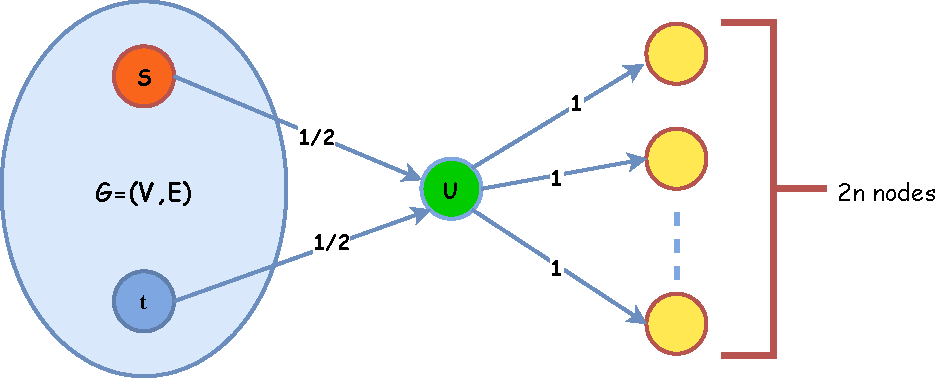
\includegraphics[height = 5 cm]{picture/reduce}
			\caption{Giản thể từ bài toán $s$-$t$ paths sang bài toán TMB.}
			\label{reduce}   
		\end{center}
	\end{figure}			
	Xem xét thể hiện $\mathcal{I}_1$ của bài toán $s$-$t$ paths, với $G = (V, E), s, t$ cho trước. Như minh họa trong hình \ref{reduce}, từ $G$, chúng ta xây dựng $G'$ như sau: Thêm đỉnh u và hai cạnh (s, u), (t, u) với trọng số $w(s, u) = w(t,u) = 1/2$, tiếp đó thêm tập $Q$ gồm 2n đỉnh và kết nối u với chúng với trọng số là 1. Với các cạnh khác, thiết lập trọng số $w = 1/\Delta$, trong đó $\Delta$ là bậc vào lớn nhất của đồ thị $G$. Chúng ta chia tất cả các đường đi bắt đầu từ $s$ thành 2 nhóm: Nhóm thứ nhất là tập tất cả các đường đi có đỉnh kết thúc thuộc tập $Q$ và nhóm thứ hai là tập còn lại. Từ công thức \eqref{inf_path}, chúng ta có: 
	\begin{align}
	\sigma_{S}(G')&=\sum_{x \in \mathsf{P}(G', s)} \prod_{e \in x}w(e)= \sum_{v \in  G' \setminus Q} \left(  \sum_{x \in \mathsf{P}(G', s, v)} \prod_{e \in x}w(e) \right) + \sum_{v \in Q} \left(  \sum_{x \in \mathsf{P}(G', s, v)} \prod_{e \in x}w(e) \right)  \nonumber
	\\
	&  =\sum_{x \in \mathsf{P}(G, s)} \prod_{e \in x}w(e) + \sum_{x \in \mathsf{P}(G', s, u)} \prod_{e \in x}w(e) + \sum_{v \in   Q } \left(  \sum_{x \in \mathsf{P}(G', s, v)} \prod_{e \in x}w(e)  \right)  \nonumber
	\\
	& = \sigma_{S}(G) +  \sum_{x \in \mathsf{P}(G', s, u)} \prod_{e \in x}w(e) +  \sum_{v \in Q } \left(  \sum_{x \in \mathsf{P}(G', s, v)} \prod_{e \in x}w(e)  \right) 
	\label{eq_1}
	\end{align}  
	và, 
	\begin{align}
	\sum_{v \in  Q } \left(  \sum_{x \in \mathsf{P}(G', s, v)} \prod_{e \in x}w(e)  \right) &= \sum_{v \in Q} \left(  \sum_{x \in \mathsf{P}(G', s, u)} w(u, v)  \prod_{e \in x}w(e)  \right) \nonumber
	\\
	& =\sum_{v \in Q} \left(  \sum_{x \in \mathsf{P}(G', s, u)} \prod_{e \in x}w(e)  \right)\ \ \ \mbox{(Vì $w(u, v)=1$)} \nonumber
	\\
	& = 2n \cdot \sum_{x \in \mathsf{P}(G', s, u)} \prod_{e \in x}w(e)
	\label{eq_3}
	\end{align}
	Từ \eqref{eq_1} và \eqref{eq_3}, chúng ta thu được:
	\begin{align}
	h(u)&= \sigma_{S}(G')- \sigma_{S}(G'\setminus \{u\})=  \sigma_{S}(G')- \sigma_{S}(G)=(2n+1)\cdot \sum_{x \in \mathsf{P}(G', s, u)} \prod_{e \in x}w(e)
	\\
	& = (2n+1)\cdot \left(  w(s, u)+ \sum_{x \in \mathsf{P}(G, s, t)} w(t, u) \prod_{e \in x}w(e) \right) 
	\\
	& = (2n+1)\cdot \left(  \frac{1}{2}+ \frac{1}{2} \sum_{x \in \mathsf{P}(G, s, t)}  \prod_{e \in x}w(e) \right)  \ \ \ \mbox{(Vì $w(s, u)= w(t, u)=\frac{1}{2}$)}
	\\
	& = \frac{2n+1}{2} \left(  \sum_{x \in \mathsf{P}(G, s, t)}  \prod_{e \in x}w(e) +1 \right) 
	\\
	& = \frac{2n+1}{2} \left(  \sum_{i=0}^{n-1} \alpha_i w^i +1 \right) 
	\end{align}   		
	với $\alpha_i=|\mathsf{P}_i(G, s, t)|$. Đặt $f(w)=\sum_{i=0}^{n-1}\alpha_i w^i$. Từ cấu trúc liên kết của G', chúng ta thấy rằng $h(u)=\max_{v \in G'}h(v)$ và $0 \leq  f(w) < 1$. Nếu có thể xác định $f(u) \geq \beta$ với $\forall \beta \in [0, 1]$ trong thời gian đa thức thì chúng ta sẽ giải được bài toán $s$-$t$ paths trong thời gian đa thức. Sử dụng tìm kiếm nhị phân trên đoạn [1, $\Delta^{n-1}$] chúng ta có thể xác định được giá trị của $f(w)$. Yêu cầu này được thực hiện trong $\mathcal{O}(\log(\Delta^{n-1}))=\mathcal{O}((n-1)\log\Delta) =\mathcal{O}(n\log n)$. Do đó việc tính toán $f(u)$ có thể thực hiện trong thời gian đa thức. Tiếp đến thay đổi trọng số w thành n giá trị phân biệt $\frac{1}{\Delta}, \frac{1}{\Delta+1}, \ldots, \frac{1}{\Delta+n-1}$, với mỗi giá trị w áp dụng phương pháp trên chúng ta thu được giá trị $f(w)$ tương ứng. Từ đó có được n phương trình $\sum_{i=0}^{n-1}\alpha_i w^i =f(w), w \in \{\frac{1}{\Delta}, \frac{1}{\Delta+1}, \ldots, \frac{1}{\Delta+n-1} \}$ với $\{\alpha_0, \alpha_2, \ldots, \alpha_{n-1}\}$ là các biến số. Ma trận tương ứng với hệ n phương trình trên là $M_{n \times n}=\{m_{ij}\}$ and $m_{ij}=w^{i} , i,j=0,..,n-1$, dễ thấy đây là ma trận Vandermonde do đó có thể dễ dàng tìm được lời giải $\{\alpha_0, \alpha_2, \ldots, \alpha_{n-1}\}$. Tổng số $s$-$t$ paths trên đồ thị G là $\sum_{i=0}^{n-1} \alpha_i$. Vì thế, nếu chúng ta xác định được $f(u) \geq \beta$ với bất kì $\beta \in [0, 1]$ trong thời gian đa thức thì sẽ giải được bài toán $s$-$t$ paths trong thời gian đa thức. 
	
	Bây giờ, xét thể hiện $\mathcal{I}_2$ của bài toán TMB trong đó $S=\{s\}$, $\gamma = \frac{2n+1}{2}(\beta+ 1) , \beta \in [0, 1]$.  Giả sử rằng $\mathcal{A}$ là một thuật toán giải quyết bài toán TMB trong thời gian đa thức. Xem xét 2 trường hợp: (1) Nếu $\mathcal{A}$ trả ra kết quả là tập $A$ có $|A|=1$, thì chúng ta chỉ cần chọn $A={u}$. Kết luận $f(w) \geq \beta$; (2) Nếu $\mathcal{A}$ trả ra kết quả tập $A$ có $|A| \ge 1$ thì ngoài $u$ sẽ cần chọn thêm một số đỉnh khác. Kết luận $f(w) < \beta$. Vì vậy $\mathcal{A}$ có thể được sử dụng để so sánh $f(w)$ với $\beta$ và có thể giải quyết bài toán $s$-$t$ paths. Điều này chỉ ra rằng bài toán TMB là khó hơn hoặc bằng bài toán $s$-$t$ paths.
\end{proof}
\subsection{Thuật toán đề xuất}
\subsubsection{Thuật toán tham lam (Greedy algorithm)}
Trong phần này chúng tôi giới thiệu một thuật toán xấp xỉ đảm bảo tỉ lệ 1 + ln($\gamma / \varepsilon$) dựa vào tính chất submodular và tính monotone của hàm h($\cdot$). Hàm $f(x)$ được gọi là hàm submodular nếu $\forall A \subset T, v \notin T$ $ f(A+ \{v\})- f(A) \geq f(T+ \{v\})- f(T)$. Còn $f(x)$ được gọi là monotone nếu $\forall T \subseteq S$ chúng ta có $f(T) \leq f(S)$.
\\
\\
\begin{algorithm}[H]			
	\KwData{Graph $G=(V,E, w)$,  $S=\{s_1, s_2, .., s_k\}$, threshold $\gamma < |V|$, parameter $\epsilon \in (0, \gamma)$} 
	\KwResult{set of nodes $A$}
	$A \leftarrow \emptyset$;
	\\
	\While{$h(A) < \gamma-\epsilon $}
	{ 	
		$u=\arg \max_{v \in V\setminus \{A \cup S\}} {h(A+ \{v\})- h(A)}$; 
		\\
		$A \leftarrow A \cup \{u\}$;
	}
	\Return $A$;
	\caption{Greedy Algorithm (GA)}
	\label{GA}
\end{algorithm}
\begin{theo}					
	Hàm $h(\cdot)$ là hàm submodular và monotone. 
	\label{sub}
\end{theo}	

\begin{proof}	
	Theo định lý 5 trong \cite{khali}, cho $A \subseteq T$ chúng ta có $h(T)-h(A)=\sigma_S(G) - \sigma_S(G \setminus T) -(\sigma_S(G) - \sigma_S(G \setminus A))  =\sigma_{S}(G \setminus A)- \sigma_{S}(G \setminus T) \geq 0$. Do đó $h(\cdot)$ là một hàm monotone. 
	
	Tiếp đến chúng ta chỉ ra rằng $\sigma_S(G \setminus A)$ là một hàm submodular với $A$ là biến số. Kí hiệu $N_E(A)$ là tập tất cả các cạnh (u, v) $\in$ E với u, v $\in$ $A$. Đặt $E_{T, v}=N_E(T+\{v\})\setminus N_E(T), E_{A, v}= N_E(A+\{v\}) \setminus N_E(A)$ dễ thấy $E_{T, v} \subseteq E_{A, v}$  nếu $A \subseteq T$ $\Rightarrow$ $N_E(A)\cup E_{T, v} \subseteq N_E(A+ \{v\})$. Lấy $\sigma_S(G \setminus N_E(X))$ là ảnh hưởng lan truyền của tập $S$ trên đồ thị $G$ sau khi loại bỏ tập cạnh $N_E(X) \subset E$, chúng ta nhận thấy $\sigma_{S}(G \setminus X)=\sigma_{S}(G \setminus N_E(X)$. Theo định lý 6 trong \cite{khali}, $\forall N_E(X) \subseteq N_E(Y), e \in N_E(Y)\setminus N_E(X)$, chúng ta có: 
	\begin{align}
	\sigma_{S}(G \setminus (N_E(X) \cup \{e\}) - \sigma_{S}(G \setminus X) 
	\leq \sigma_{S}(G \setminus (N_E(Y) \cup \{e\})) - \sigma_{S}(G \setminus Y)
	\label{super}
	\end{align}
	Vì thế,
	\begin{align}
	\sigma_{S}(G \setminus A)-\sigma_{S}(G \setminus (A \cup \{v\})) 
	& =\sigma_{S}(G \setminus N_E(A))-\sigma_{S}(G \setminus N_E(A+\{v\})) 
	\\
	&	\geq \sigma_{S}(G \setminus N_E(A))-\sigma_{S}(G \setminus (N_E(A) \cup E_{T, v})) 
	\\
	&	\geq \sigma_{S}(G \setminus N_E(T))-\sigma_{S}(G \setminus (N_E(T) \cup E_{T, v}))  
	\\
	& = \sigma_{S}(G\setminus T)-\sigma_{S}(G \setminus (T \cup \{u\}))  (\mbox{Theo BĐT \eqref{super}})
	\end{align}
	Kết hợp với công thức $h(A)= \sigma_S(G)- \sigma_S(G\setminus A)$ chúng ta có được $h(\cdot)$ là một hàm submodular.
\end{proof}

\begin{theo} Với $\forall$ $\epsilon \in (0, \gamma)$, thuật toán \ref{GA} đưa ra lời giải $A$ thỏa mãn $h(A) \geq \gamma- \epsilon$, và $|A|$ là không vượt quá tích của $1+\ln(\gamma/ \epsilon)$ với số đỉnh của lời giải tối ưu \label{app}
\end{theo}		
\begin{proof}
	Chi tiết cách chứng minh định lý \ref{app} được chỉ ra trong \cite{snam}. 
\end{proof}
Thuật toán tham lam có cách tiếp cận khá đơn giản là mỗi bước tìm đỉnh $u$ sao cho hàm $h(A)$ tăng nhiều nhất. Song vấn đề khó khăn nhất gặp phải là tính giá trị hàm $\sigma(\cdot)$ có độ khó là $\#P-\text{khó}$, chứng minh trong \cite{vali}. Vì vậy chúng tôi đưa ra một thuật toán hiệu quả trong phần sau.

\subsubsection{Thuật toán STMB (STMB algorithm)}
Thuật toán tham lam đưa ra một lời giải tốt xong lại không đảm bảo yêu cầu về thời gian với dữ liệu lớn do đó trong phần này chúng tôi đưa ra một giải pháp đảm bảo yêu cầu cả về chất lượng lời giải cũng như thời gian tính toán. Dưới đây là các bước chính trong thuật toán chúng tôi đề xuất:
\begin {itemize}
\item Đầu tiên sáp nhập các đỉnh trong tập nguồn S thành một nút I bằng cách áp dụng thuật toán \ref{MERGE} được đề xuất bởi Zhang \cite{yao16}. Chúng ta thu được một đồ thị mới và nguồn phát tán thông tin sai lệch bây giờ chỉ còn là một đỉnh I duy nhất.
\end{itemize}
\begin{algorithm}[H]			
\KwData{Graph $G=(V,E, w)$,  $S=\{s_1, s_2, .., s_k\}$} 
\KwResult{Graph $G'=(V', E', w')$, I}
$G' \leftarrow G$;
\\
Add node I to G'			
\\
\ForEach{s $\in$ S}
{
	\If{$\exists$ (s, v) }
	{
		\eIf{(I, v) $\notin$ G'}
		{
			Add edge (I, v) to G'
			\\
			w'(I, v) = w(s, v)
		}
		{
			w'(I, v) = w'(I, v) + w(s, v)
		}
		Remove (s,v) from G'
	}
}
Remove all node in S from G'
\\
\Return G', I;
\caption{MERGE Algorithm(MERGE)}
\label{MERGE}
\end{algorithm}	
\begin {itemize}			
\item Tiếp đến chúng tôi tạo ra $\mu(\mu \in N*)$ đồ thị mẫu g từ G' bằng cách: mỗi đỉnh v $\in$ V chọn nhiều nhất một đỉnh kề đi đến nó một cách ngẫu nhiên sao cho xác suất chọn cạnh (u, v) là w(u, v) và xác suất không chọn cạnh nào là 1 - $\sum_{u} w(u, v)$. Những cạnh được chọn được gọi là cạnh sống  (live - edge) và tất cả các cạnh còn lại được gọi là cạnh bị chặn (blocked-edge). Chi tiết cách lấy đồ thị mẫu được mô tả trong thuật toán \ref{GSGLT} và trong hình \ref{example}: 
\end {itemize}
\begin{figure}[H]
\subfloat[Đồ thị $G'$ sau khi hợp nhất các đỉnh trong nguồn S\label{fig:test1}]
{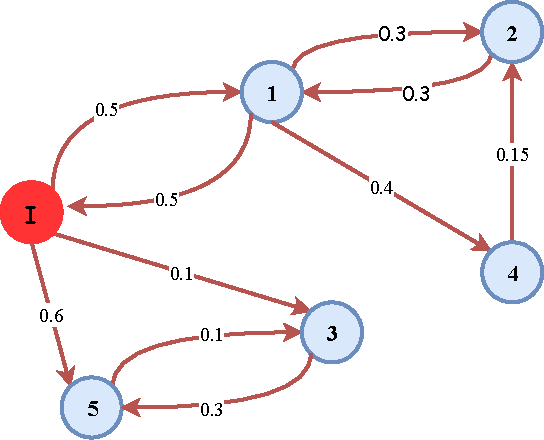
\includegraphics[width=.3\linewidth]{picture/1}}\hfill
\subfloat[Đồ thị mẫu $g$\label{fig:test2}]
{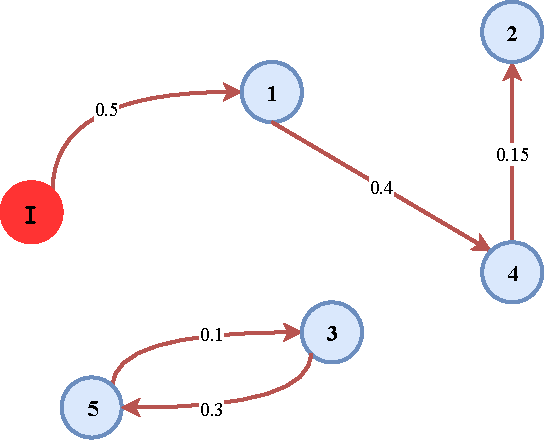
\includegraphics[width=.3\linewidth]{picture/2}}\hfill
\subfloat[Cây gốc $I$ tạo ra từ $g$ \label{fig:test3}]
{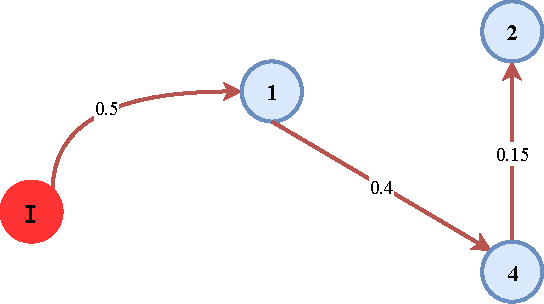
\includegraphics[width=.3\linewidth]{picture/3}}
\caption{Ví dụ tạo ra một cây gốc $I$ từ $G$ trên mô hình LT}
\label{example}
\end{figure}	
\begin{algorithm}[H]
\KwData{Graph G=(V,E, w), I} 
\KwResult{Tree g root at I}			
g $\Leftarrow \emptyset$
\\
\For{$v \in V_G$}
{	
	$\gamma_{active} \leftarrow$ random(0, 1)
	\\
	sum\_weight $\leftarrow$ 0
	\\
	\For{u $\in$ in\_neighbors(v)}
	{
		sum\_weight += w(u, v)
		\\
		\If{sum\_weight $\geq \gamma_{active}$}
		{
			Add edge (u, v) to g
			\\
			Break
		}
	}
}		
g $\leftarrow$ DFS$_{tree}$(I,g)
\\
\Return g
\caption{Get Sample Graph LT Algorithm (GSG\_{LT})}
\label{GSGLT}
\end{algorithm}	
\begin {itemize}
\item Trên cây T$_{I}^i$, ảnh hưởng địa phương của nút v là số nút con của cây gốc v kể cả v trên cây T$_{I}^i$. Áp dụng thuật toán DFS dễ dàng tìm được số nút con của v. Ảnh hưởng giảm của nguồn S khi loại đỉnh u khỏi G bằng lượng ảnh hưởng giảm trung bình khi loại u trên tất cả các cây T$_{I}^i$. Kí hiệu h(u, $T_I^i$) là lượng ảnh hưởng giảm trên cây $T_I^i$ sau khi loại bỏ đỉnh u khỏi $T_I^i$. Áp dụng phương pháp Lazy forward của Leskovec \cite{lazy} để tìm kiếm lời giải. 
\end {itemize}
\begin{algorithm}[H]
%\SetAlgoNlRelativeSize{0}
\KwData{Graph $G=(V,E, w)$,  $\mathcal{S}=\{s_1, s_2, .., s_q\}$, threshold $\gamma>0$} 
\KwResult{set of nodes $A$}
$A \leftarrow \emptyset$;	$(G', I) \leftarrow \mathtt{Merge}(G, \mathcal{S})$.
\\
Remove all node, $I$ can't reach in $G$.
\\
Generate $\eta$ sample graphs and set $\eta$ trees $\mathcal{L}=\{T_{I}^1, T_{I}^2, \ldots, T_{I}^{|\mathcal{\eta}|}\}$
\\
For each $ T_{I} \in \mathcal{L}$, calculate $h(u, T_{I})$ for all $u \in T_{I}$ (by using DFS algorithm).
\\
\For{$u \in V$}
{
	$u.\delta(u) \leftarrow \frac{1}{\eta}\sum_{T_{I} \in \mathcal{L}} h(u, T_{I})$; $u. cur \leftarrow 1$
	\\
	Insert element $u$ into $Q$ with $u.\delta(u)$ as the key
}
$ h_{max} \leftarrow 0$; $iteration \leftarrow 1$
\\
\While{$ h_{max} <\gamma-\epsilon $}
{
	$u_{max} \leftarrow  dequence \  Q$
	\\
	\eIf{$u_{max}.cur =iteration$}
	{
		$A \leftarrow A \cup \{u_{max}\}$ ; $iteration \leftarrow iteration+1 $
		\\
		\ForEach{$T_{I} \in \mathcal{L}_c $}
		{
			If $u_{max} \in T_{I}$, remove node $u_{max}$ and update $h(v, T_{I})$, $ \forall v \in T_{I}$.
		}
		$h_{max} \leftarrow h_{max}+ u_{max}.\delta(u_{max})$
	}
	{
		$u_{max}. \delta(u_{max}) \leftarrow  \frac{1}{\eta}\big(\sum_{T_{I} \in \mathcal{L}}h(I, T_{I}) - \sum_{T_{I} \in \mathcal{L}} h(I, T_{I} \setminus u_{max})\big)$
		\\
		$u_{max}. cur =iteration$; re-insert $u_{max}$ into $Q$
	}
}
\Return $A$;
\caption{Scalable $\mathsf{TMB}$ for LT model ($\mathsf{TMB}$) Algorithm}
\label{STMB}
\end{algorithm}				
{\itshape Độ phức tạp của thuật toán: }		
Để đánh giá độ phức tạp của thuật toán trước tiên chúng ta đi phân tích độ phức tạp của các thuật toán con trong nó.
\begin {itemize}
\item Thuật toán MERGE có độ phức tạp là O(k + | N$_{in}(S)$ |).

\item Quá trình tạo ra $\mu$ đồ thị mẫu dòng 3 có độ phức tạp O($\mu(m + n)$).

\item Do T$_{I}^i$ là một cây nên việc tính toán h(u, T$_{I}^i$) $\forall u \in \text{T}_{I}^i$ mất O$(\mu n)$ 

\item Phần Lazy Forward có độ phức tạp là O(qmn) với q là số vòng lặp từ dòng 10 đến 23.
\end {itemize}

Vậy nên toàn bộ thuật toán TMB có độ phức tạp là O($\mu$(m+qn)).

\subsection{Kết quả thực nghiệm với dữ liệu đã công bố}	

Trong mục này chúng tôi đưa ra kết quả thực nghiệm của thuật toán STMB với 3 bộ dữ liệu đã công bố của các mạng xã hội và so sánh về chất lượng lời giải, tốc độ thực hiện với một số thuật toán cơ bản khác.
Thuật toán được thực hiện bằng ngôn ngữ Python 2.7, sử dụng thư viện hỗ trợ NetworkX\footnote{Hướng dẫn sử dụng https://networkx.github.io/} và chạy trên máy Linux Server với cấu hình 2.30 GHz Intel\textsuperscript{\textregistered} Xeon\textsuperscript{\textregistered} CPU E5-2697, bộ nhớ 128G of RAM DDR4.
\subsubsection{Dữ liệu}
Với mục đích thực nghiệm, chúng tôi sử dụng 3 bộ dữ liệu mạng thực tế thu thập trên trang snap.stanford.edu \footnote{https://snap.stanford.edu/data/index.html}, Một vài thông tin cơ bản về chúng được đưa ra trong bảng \ref{TMB:table}. 
\begin{table}[h]
	\centering
	\begin{tabular}{|c|c|c|c|}
		\hline 
		Mạng & NetS & AS & NetHEPT\\ 
		\hline 
		Số đỉnh & 1.5K & 6.4K & 15.2K \\ 
		\hline 
		Số cạnh & 5.4K & 12.5K & 32.2K\\ 
		\hline 
		Bậc trung bình & 3.8 & 7.5 & 4.2\\ 
		\hline 
		Số đỉnh nguồn & 100 & 300 & 1000\\ 
		\hline 
	\end{tabular} 
	\caption{Các bộ dữ liệu dùng trong thực nghiệm với giải pháp TMB}
	\label{TMB:table}
\end{table}

\texttt{NetS}\cite{NetS}: Một mạng lưới các nhà khoa học làm việc trên lý thuyết và thử nghiệm mạng, được biên soạn vào tháng 5/2006.

\texttt{AS}\cite{AS}: Biểu đồ các bộ định tuyến bao gồm Internet có thể được sắp xếp thành các biểu đồ con được gọi là Autonomous Systems(AS). Mỗi AS trao đổi lưu lượng với một số hàng xóm (peer). Chúng ta có thể xây dựng một mạng lưới các AS liên kết với nhau dựa trên nhật ký Border Gateway Protocol (BGP). Bộ dữ liệu là kết quả từ dự án University of Oregon Route Views. 

\texttt{NetHEPT}\cite{kemple1, chen10LT}: Một mạng lưới hợp tác học thuật được trích xuất từ phần "High Energy Physics-Theory" của trang điện tử arXiv\footnote{https://arxiv.org/} trong khoảng thời gian từ năm 1991--2003. Mỗi đỉnh trong mạng đại diện cho một tác giả và mỗi cạnh kết nối 2 đỉnh cho biết 2 tác giả đã đồng tác giả của một bài báo.

\subsubsection{Thiết lập tham số}
Chúng tôi sử dụng các thiết lập tham số dưới đây cho việc đánh giá thực nghiệm:
Theo các nghiên cứu trước \cite{khali, kemple1,chen10LT}, chúng tôi thiết lập trọng số các cạnh của đồ thị trên mô hình LT theo công thức $w(u,v) = 1/N_{in}(v)$. Với nguồn phát tán thông tin sai lệch chúng tôi chọn ngẫu nhiên từ 4-6\% số lượng đỉnh của cả đồ thị, phụ thuộc vào kích thước của đồ thị. 


\subsubsection{Các thuật toán sử dụng}
Trong thực nghiệm, chúng tôi so sánh thuật toán STMB với một số thuật toán sau, các thuật toán này thường được sử dụng trong các nghiên cứu liên quan về vấn đề nhóm tác giả nghiên cứu:
\begin {itemize}
\item PageRank: Tính toán ranking của các đỉnh trong đồ thị $G$ dựa vào cấu trúc các cạnh liên kết với nó. Đây là thuật toán được thiết kế để xếp hạng các trang web từ đó đưa ra kết quả tìm kiếm. Do $h(\cdot)$ là hàm monotone nên sau khi sắp xếp hạng của các đỉnh trong đồ thị, chúng tôi sử dụng thuật toán tìm kiếm nhị phân để tìm kiếm tập lời giải A với |A| đỉnh có rank lớn nhất.
\item High-Degree: Một thuật toán heuristic dựa vào bậc của một đỉnh. Bậc của một đỉnh ở đây là tổng số đỉnh được tính theo công thức $d(v) = N_{in}(v) + N_{out}(v)$. Tương tự như thuật toán PageRank sau khi sắp xếp các đỉnh dựa trên bậc của chúng, chúng tôi sử dụng thuật toán tìm kiếm nhị phân để tìm lời giải cho bài toán.
\item Greedy: Thuật toán Greedy đưa ra trong thuật toán \ref{GA} kết hợp với các tối ưu trong \cite{Jleskovec} giúp tăng tốc độ thuật toán song không làm ảnh hưởng đến chất lượng lời giải.
\end{itemize} 

\subsubsection{Kết quả thực nghiệm} 
Như mô tả trong hình \ref{solSTMB}, số lượng đỉnh được chọn đưa ra bởi thuật toán STMB là nhỏ nhất. STMB tốt hơn lên đến 39\% so với thuật toán Greedy, hơn 60\%-95\% và 57\%-87\% so với thuật toán PageRank và High-Degree tương ứng. Để kiểm tra kết quả thu được từ thuật toán STMB, chúng tôi chạy 10000 mẫu Monte-Carlo để ước lượng giá trị của hàm $h(A)$ và kết quả kiểm tra được đưa ra trong hình \ref{check}. Trong hầu hết các trường hợp $h(A)$ vượt qua ngưỡng yêu cầu.
\begin{figure}[H]
\begin{tabular}{lll}
	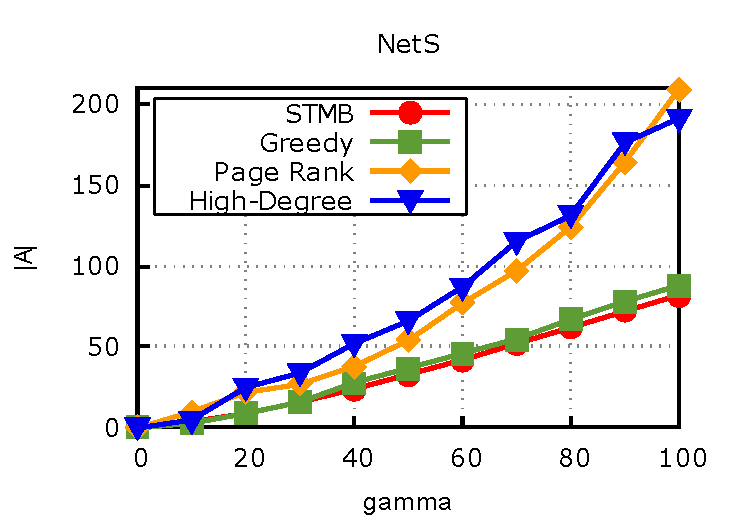
\includegraphics[height = 3.2cm]{picture/NetS} &
	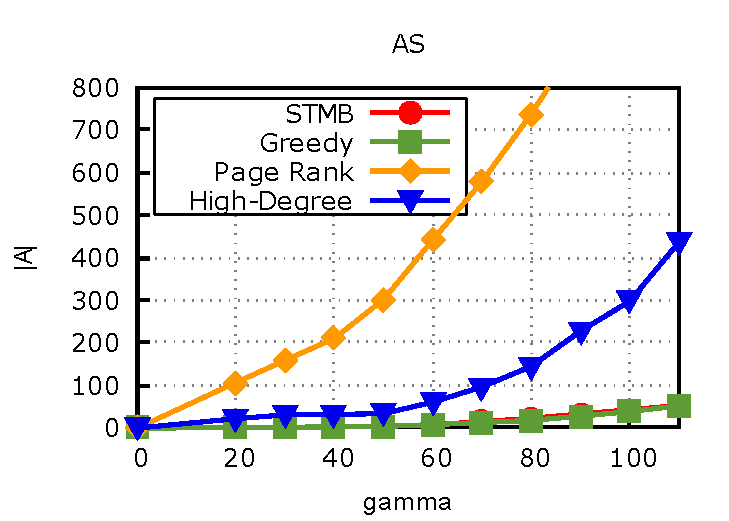
\includegraphics[height = 3.2cm]{picture/AS} &   
	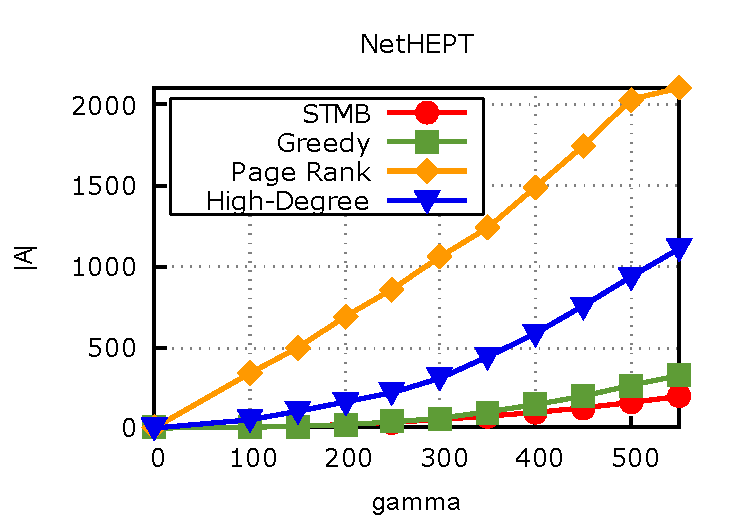
\includegraphics[height = 3.2cm]{picture/NetHEPT}
	\\
	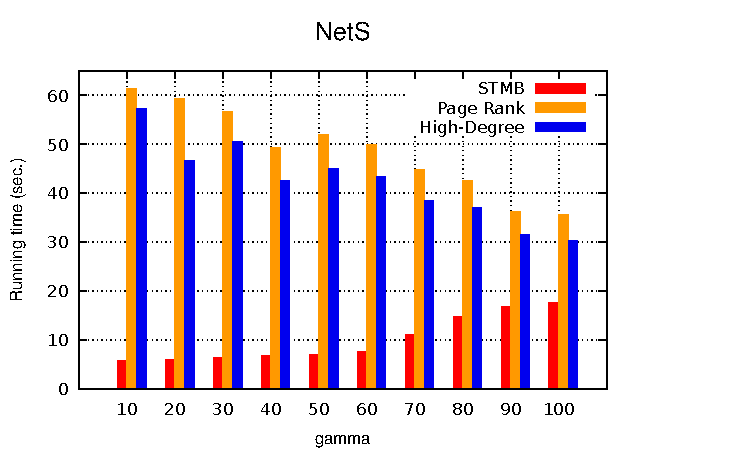
\includegraphics[height = 3.2cm]{picture/TimeNetS} &
	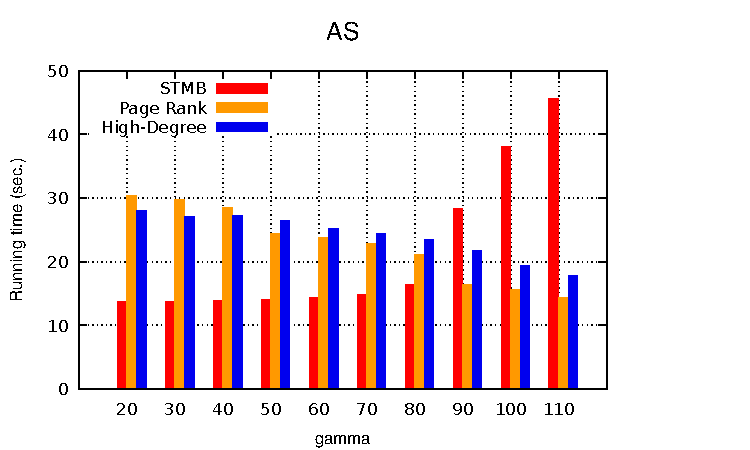
\includegraphics[height = 3.2cm]{picture/TimeAS} &   
	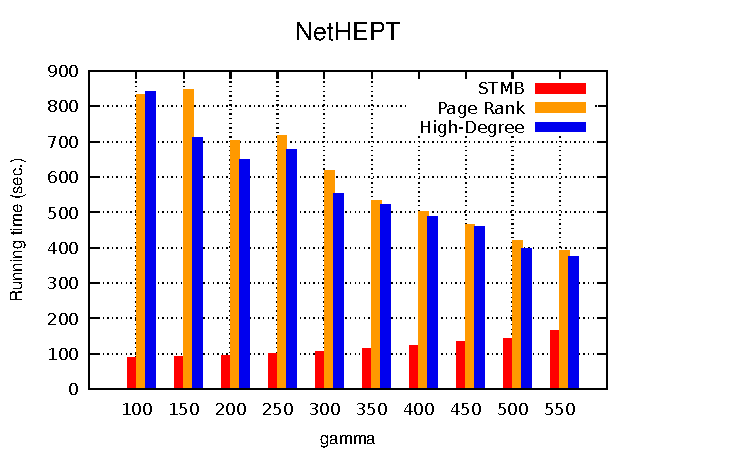
\includegraphics[height = 3.2cm]{picture/TimeNetHEPT}
\end{tabular}
\caption{So sách chất lượng lời giải và thời gian chạy của các thuật toán cho bài toán TMB}
\label{solSTMB}    
\end{figure}
\begin{figure}[H]
\begin{tabular}{ccc}
	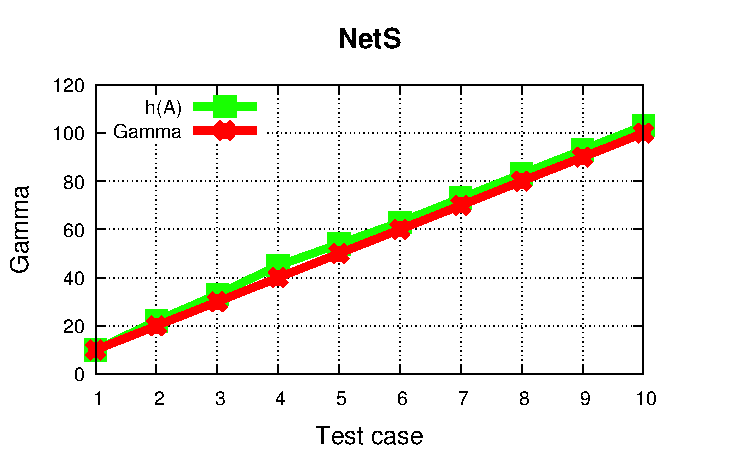
\includegraphics[height = 3.2 cm]{picture/CheckNetS} &
	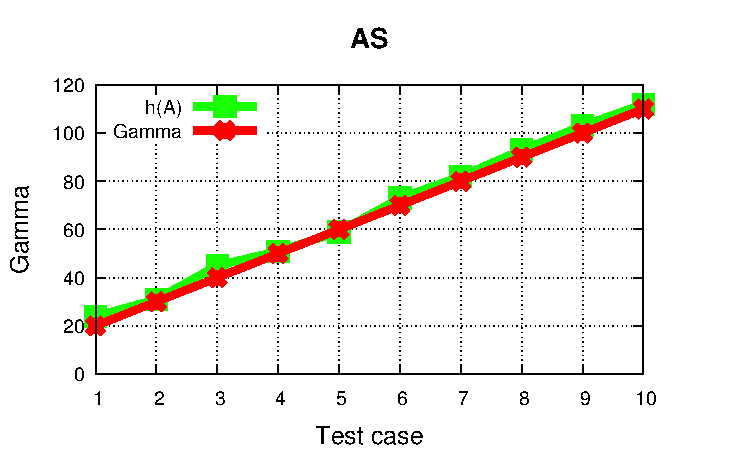
\includegraphics[height = 3.2 cm]{picture/CheckAS} &   
	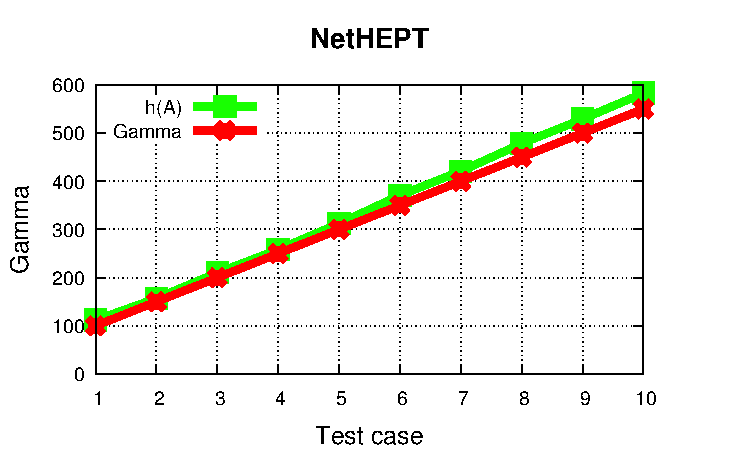
\includegraphics[height = 3.2 cm]{picture/CheckNetHEPT}
\end{tabular}
\caption{Kiểm tra kết quả của thuật toán STMB}
\label{check}    
\end{figure}
\begin{table}[h]
\label{tab:time}       % Give a unique label
% For LaTeX tables use
\begin{center}
	\begin{tabular}{|c|c|c|c|c|}				
		\hline 
		\textbf{} & {$\mathsf{STMB}$} & {$\mathsf{Greedy}$} & {Page Rank} & {High-Degree} 				
		\\ 
		\hline 
		NetS & \textbf{17.57(s)} &	14206.80(s) &	35.73(s) &	30.24(s)
		\\ 
		\hline 
		AS & 45.70(s) & 14074.87(s) & \textbf{14.39(s)} &	17.85(s)
		\\
		\hline 
		NetHEPT & \textbf{165.12(s)} & 582566.74(s) & 392.34(s) & 374.66(s)
		\\
		\hline 
	\end{tabular}
\end{center}
\caption{So sánh thời gian chạy của các thuật toán với trường hợp $\gamma$ lớn nhất}
\label{timeSTMB}
\end{table}
Thời gian chạy của các thuật toán trên 3 bộ dữ liệu trong trường hợp có $\gamma$ là lớn nhất được đưa ra trong bảng \ref{timeSTMB} cho thấy thuật toán Greedy có chất lượng lời giải tương đương với thuật toán STMB song thời gian thực nghiệm trên các bộ dữ liệu lại rất không hiệu quả. Trong khi đó thuật toán STMB có thời gian thực hiện khá là nhanh, không khác biệt nhiều so với các thuật toán cơ bản song vẫn đảm bảo có một lời giải tốt.

\bibliographystyle{plain}
\begin{thebibliography}{4}
	%chapter 1
	\bibitem{quidinh} Quy định việc cung cấp, sử dụng Internet của chính phử. Truy xuất từ: https://thuvienphapluat.vn/van-ban/Cong-nghe-thong-tin/Nghi-dinh-72-2013-ND-CP-quan-ly-cung-cap-su-dung-dich-vu-Internet-va-thong-tin-tren-mang-201110.aspx. 
	\bibitem{karlova1} Karlova, Natascha, Fisher Karen. A Social Diffusion Model of Misinformation and Disinformation for Understanding Human Information Behaviour. Information Research, 2013, pp. 1-17.
	\bibitem{APhack}Tin tặc giả mạo đăng tin sai lêch trên hãng thông tấn Associated Press. Truy xuấttừ:https://www.usatoday.com/story/theoval/2013/04/23/obama-carney-associated-press-hack-white-house/2106757
	\bibitem{Anhhuong} Ảnh hưởng của MXH với bầu cử Pháp. Truy xuất từ:  https://baomoi.com/facebook-va-phep-thu-mang-ten-bau-cu-phap/c/22045463.epi.
	\bibitem{ebola} Tin đồn dịch Ebola bùng phát tại Hà Nôi. Truy xuất từ: http://baophapluat.vn/tin-nong/lam-ro-danh-tinh-2-nguoi-tung-tin-don-that-thiet-ve-benh-dich-ebola-194152.html
	\bibitem{formusa} Tin đồn công ty Formusa xả thải chưa qua xử lí. Truy xuất từ: http://m.vietnamnet.vn/vn/thoi-su/moi-truong/bo-tn-mt-bac-bo-tin-don-formosa-phat-thai-dioxin-370436.html
	\bibitem{dieuduong} Phóng sự về nghề điều dưỡng viên xuất khẩu lao động tại Đức. Truy xuất từ: https://baomoi.com/du-hoc-sinh-duc-phan-doi-phong-su-cua-vtv-ve-nghe-dieu-duong-vien-luong-thang-100-trieu/c/21365466.epi
	
	%chapter 2
	\bibitem{zhang1} H Zhang, M. Alim, M. T. Thai, and H. Nguyen, Monitor Placement to Timely Detect Misinformation in Online Social Networks, in Proceedings of the 2015 IEEE International Conference on Communications (ICC), 2015.
	\bibitem{kemple1} D. Kempe, J. Kleinberg, and E. Tardos. 2003. Maximizing the spread of influence through a social network. In Proceedings of the ninth ACM SIGKDD international conference on Knowledge discovery and data mining. Washington, DC, USA, 137-146. https://doi.org/10.1145/956750.956769. 
	\bibitem{kemple2} D. Kempe, J. Kleinberg, and E. Tardos. Influential Nodes in a Diffusion Model for Social Networks. In ICALP, 2005, pp. 1127-1138.
	\bibitem{Golden} J. Goldenberg, B. Libai, and E. Muller. Talk of the Network: A Complex Systems Look at the Underlying Process of Word-of-Mouth. Marketing Letters, 2001, pp. 211-223
	\bibitem{Carnes} T. Carnes, R. Nagarajan, S. M. Wild, and A. V. Zuylen. Maximizing Influence in a Competitive Social Network: a Follower’s Perspective. In Proceedings of the Ninth International Conference on Electronic Commerce, 2007, pp. 351-360.
	\bibitem{leskovec} J. Leskovec, M. Mcglohon, C. Faloutsos, N. Glance, and M. Hurst. Cascading Behavior in Large Blog Graphs. In Proceedings of the 2007 SIAM International Conference on Data Mining, 2007, pp. 551-556.
	\bibitem{pedro} Pedro Domingos and Matthew Richardson. Mining the Network Value of Customers. In Proceedings of the Seventh ACM SIGKDD International Conference on Knowledge Discovery and Data Mining, 2001, pp. 57-66.
	\bibitem{leskovec} J. Leskovec, A. Krause, C. Guestrin, C. Faloutsos, J. M. Van–Briesen, and N. S. Glance.: Cost–effective outbreak detection in networks. In: Proceedings of the 13th ACM SIGKDD international conference on Knowledge discovery and data mining, 420-429, ACM (2007).
	\bibitem{goyal} A. Goyal, W. Lu, L. V.S. Lakshmanan. Celf++: Optimizing the Greedy Algorithm for Onfluence Maximization in Social Networks. In Proc. WWW, 2011, pp. 47-48.
	\bibitem{snam} A. Goyal, F. Bonchi, L. V. S. Lakshmanan, and S. Venkatasubramanian.: On minimizing budget and time in influence propagation over social networks. Social Network Analysis and Mining, 2(1), 179--192 (2012)
	\bibitem {chen} Wei Chen, Laks V.S. Lakshmanan, and Carlos Castillo. Information and Influence Propagation in Social Networks. A Publication in the Morgan \& Claypool Publishers series Synthesis Lectures on Data Management, 2014.
	\bibitem{qazvin} V. Qazvinian, E. Rosengren, D. R. Radev, and Qiaozhu Mei. Rumor has it: Identifying Misinformation in Microblogs. In Proc. EMNLP, 2011, pp. 1589-1599.
	\bibitem{kwon} S. Kwon, M. Cha, K. Jung, W. Chen, and Y. Wang. 2013. Prominent Features of Rumor Propagation in Online Social Media. In Proc. ICDM, 2013, pp. 1103-1108.
	\bibitem{nguyen1} D. T. Nguyen, N. P. Nguyen, and M. T. Thai. Sources of Misinformation in Online Social Networks: Who to Suspect. In Proceedings of the IEEE Military Communications Conference, 2012.
	\bibitem{nguyen9} Nam P. Nguyen, Guanhua Yan, My T. Thai (2013), "Analysis of misinformation containment in online social networks", Computer Networks.
	\bibitem{nguyen30} D. T. Nguyen, N. P. Nguyen, and M. T. Thai. Sources of Misinformation in Online Social Networks: Who to Suspect. In Proceedings of the IEEE Military Communications Conference, 2012.
	\bibitem{ceren} Ceren Budak, Divyakant Agrawal, Amr El Abbadi, Limiting the Spread of Misinformation in Social Networks.
	\bibitem{zhang31} Huiling Zhang, Md Abdul Alim, Xiang Li, My T. Thai, and Hien T. Nguyen. 2016. Misinformation in online social networks: Detect them all with a limited budget. ACM Trans. Inf. Syst. 34, 3, Article 18 (April 2016), 24 pages. DOI:http://dx.doi.org/10.1145/2885494.
	
	%chapter 3
	\bibitem{zhang32} Zhang Y, Prakash B (2015) Data-aware vaccine allocation over large networks. ACM Trans Knowl Discov Data. https://doi.org/10.1145/2803176.
	\bibitem{zhang33} Zhang H, Alim M, Li X, My TT, Nguyen H (2016a) Misinformation in online social networks: catch them all with limited budget. ACM Trans Inf Syst 34(3):18.
	\bibitem{zhang34} Zhang Y, Adigay A, Saha S, Vullikanti A, Prakash A (2016b) Near-optimal algorithms for controlling propagation at group scale on networks. IEEE Trans Knowl Data Eng. https://doi.org/10.1109/TKDE. 2016.2605088
	\bibitem{twitter} Yadron D (2017) Twitter deletes 125,000 Isis accounts and expands anti-terror teams. The Guardian Web. https://www.theguardian.com/technology/2016/feb/05/ twitter-deletes-isis-accounts-terrorismonline. Accessed 24 June 2017.
	\bibitem{french}  Kottasov I (2017) Facebook targets 30,000 fake accounts in France. CNN media Web. http://money.cnn. com/2017/04/14/media/facebook-fake-news-france-election/index.html. Accessed 24 June 2017.
	\bibitem{zaixin} Zaixin Lu, Wei Zhang, Weili Wu, Joonmo Kim, and Bin Fu. 2011. The complexity of influence maximization problem in the deterministic linear threshold model. Journal of Combinatorial Optimization 24, 3 (April 2011), 374–378. https://doi.org/10.1007/s10878-011-9393-3. 
	\bibitem{vijay38} Vijay V. Vazirani. 2001. Approximation Algorithms. Springer, Verlag New York, Inc. New York, NY, USA.
	\bibitem{vali} L. G. Valiant.: The complexity of enumeration and reliability problems. SIAM Journal on Computing 8(3), 410--421 (1979)
\end{thebibliography}

\backmatter %Định dạng các trang cuối, số thứ tự được đánh kiểu ả rập: 1,2,3...

%\begin{multicols}{2}
\printindex
%\end{multicols}

%Các tùy biến của định dạng trang được tìm và định nghĩa lại ở mybook.cls, chú ý tìm từ khóa.
\end{document}